\documentclass[a4paper,twoside,openright,makeidx,12pt]{book}
%\usepackage{draftcopy}
%%$Id: macro.tex,v 1.10 2004/12/08 13:38:58 acary Exp $


%\usepackage{a4wide}
\textheight 25cm
\textwidth 16.5cm
\topmargin -1cm
%\evensidemargin 0cm
\oddsidemargin 0cm
\evensidemargin0cm
\usepackage{layout}


\usepackage{amsmath}
\usepackage{amssymb}
\usepackage{minitoc}
%\usepackage{glosstex}
\usepackage{colortbl}
\usepackage{hhline}
\usepackage{longtable}

%\usepackage{glosstex}
%\def\glossaryname{Glossary of Notation}
\def\listacronymname{Acronyms}

\usepackage[outerbars]{changebar}\setcounter{changebargrey}{20}
%\glxitemorderdefault{acr}{l}

%\usepackage{color}
\usepackage{graphicx,epsfig}
\graphicspath{{./Figures/}}
\usepackage[T1]{fontenc}
\usepackage{rotating}

%\usepackage{algorithmic}
%\usepackage{algorithm}
\usepackage{ntheorem}
\usepackage{natbib}


%\renewcommand{\baselinestretch}{2.0}
\setcounter{tocdepth}{2}     % Dans la table des matieres
\setcounter{secnumdepth}{3}  % Avec un numero.



\newtheorem{definition}{Definition}
\newtheorem{lemma}{Lemma}
\newtheorem{claim}{Claim}
\newtheorem{remark}{Remark}
\newtheorem{assumption}{Assumption}
\newtheorem{example}{Example}
\newtheorem{conjecture}{Conjecture}
\newtheorem{corollary}{Corollary}
\newtheorem{OP}{OP}
\newtheorem{problem}{Problem}
\newtheorem{theorem}{Theorem}


\newcommand{\CC}{\mbox{\rm $~\vrule height6.6pt width0.5pt depth0.25pt\!\!$C}}
\newcommand{\ZZ}{\mbox{\rm \lower0.3pt\hbox{$\angle\!\!\!$}Z}}
\newcommand{\RR}{\mbox{\rm $I\!\!R$}}
\newcommand{\HH}{\mbox{\rm $I\!\!H$}}
\newcommand{\NN}{\mbox{\rm $I\!\!N$}}

\newcommand{\Mnn}{\mathcal M^{n\times n}}
\newcommand{\Mnp}[2]{\ensuremath{\mathcal M^{#1\times #2}}}



\newcommand{\Frac}[2]{\displaystyle \frac{#1}{#2}}

\newcommand{\DP}[2]{\displaystyle \frac{\partial {#1}}{\partial {#2}}}

% c++ variables writting
\newcommand{\varcpp}[1]{\textit{#1}}
% itemize
\newcommand{\bei}{\begin{itemize}}
\newcommand{\ei}{\end{itemize}}

\newcommand{\ie}{i.e.}
\newcommand{\eg}{e.g.}
\newcommand{\cf}{c.f.}
\newcommand{\putidx}[1]{\index{#1}\textit{#1}}

\def\Er{{\rm I\! R}}
\def\En{{\rm I\! N}} 
\def\Ec{{\rm I\! C}}
 
\def\zc{\hat{z}}
\def\wc{\hat{w}}

\font\tete=cmr8 at 8 pt


% normal tangent
\def\n{{\hbox{\tiny{N}}}}
\def\t{{\hbox{\tiny{T}}}}
\def\nt{\hbox{\tiny{NT}}}
\def\nsf{\hbox{\tiny{\textsf N}}}
\def\tsf{\hbox{\tiny{\textsf T}}}
\def\sigman{\sigma_{\n}}
\def\sigmat{\sigma_{\t}}
\def\sigmant{\sigma_{\nt}}
\def\epsn{\epsilon_{\n}}
\def\epst{\epsilon_{\t}}
\def\epsnt{\epsilon_{\nt}}
\def\eps{\epsilon}
\def\veps{\varepsilon}
\def\sig{\sigma}
\def\Rn{R_{\n}}
\def\Rt{R_{\t}}
\def\cn{c_{\n}}
\def\Cn{C_{\n}}
\def\ct{c_{\t}}
\def\Ct{C_{\t}}
\def\un{u_{\n}}
\def\ut{\buu_{\t}}
\def\uut{u_{\t}}
\def\unc{u_{\n}^c}
\def\utc{\buu_{\t}^c}
\def\vn{v_{\n}}
\def\vt{v_{\t}}
\def\rr{\hbox{\tiny{\textsf R}}}
\def\irr{\hbox{\tiny{\textsf{IR}}}}
\def\rn{r_{\n}}
\def\rt{\brr_{\t}}
\def\rnc{r_{\n}^c}
\def\rtc{\brr_{\t}^c}
\def\trn{\Tilde{r}_{\n}}
\def\trt{\Tilde{\brr}_{\t}}
\def\tr{\Tilde{\brr}}
\def\tv{\Tilde{\bvv}}
\def\vn{v_{\n}}
\def\vt{\bvv_{\t}}
\def\adh{\mathsf{adh}}
\def\adj{\hbox{\tiny{\textsf{adj}}}}
\def\adjc{\hbox{\tiny{\textsf{adjC}}}}
\def\adja{\hbox{\tiny{\textsf{adjA}}}}
\def\cc{\hbox{\tiny{\textsf C}}}
\def\ca{\hbox{\tiny{\textsf A}}}

\DeclareMathOperator{\proj}{proj}
\DeclareMathOperator{\expm}{expm}
\DeclareMathOperator{\dexp}{dexp}
\DeclareMathOperator{\dlexp}{d^l exp}
\DeclareMathOperator{\drexp}{d^r exp}
\DeclareMathOperator{\dexpm}{dexpm}
\DeclareMathOperator{\expq}{expq}
\DeclareMathOperator{\dexpq}{dexpq}
\DeclareMathOperator{\Ad}{Ad}
\DeclareMathOperator{\ad}{ad}
\DeclareMathOperator{\dd}{d}



%%  Les ensembles de nombres  C. Fiorio (fiorioÊatÊmath.tu-berlin.de) 
%
\def\nbR{\ensuremath{\mathrm{I\!R}}} % IR
\def\nbN{\ensuremath{\mathrm{I\!N}}} % IN
\def\nbF{\ensuremath{\mathrm{I\!F}}} % IF
\def\nbH{\ensuremath{\mathrm{I\!H}}} % IH
\def\nbK{\ensuremath{\mathrm{I\!K}}} % IK
\def\nbL{\ensuremath{\mathrm{I\!L}}} % IL
\def\nbM{\ensuremath{\mathrm{I\!M}}} % IM
\def\nbP{\ensuremath{\mathrm{I\!P}}} % IP

%----------------------------------------------------------------------
%                  Modification des subsubsections
%----------------------------------------------------------------------
\makeatletter
\renewcommand\thesubsubsection{\thesubsection.\@alph\c@subsubsection}
\makeatother

%----------------------------------------------------------------------
%             Redaction note environnement
%----------------------------------------------------------------------
\makeatletter
\theoremheaderfont{\scshape}
\theoremstyle{marginbreak}
\theorembodyfont{\upshape}
%\newtheorem{rque}{\bf Remarque}[chapter]
%\newtheorem{rque1}{\bf \fsc{Remarque}}[chapter] !!! \fsc est une commande french
\newtheorem{ndr1}{\textbf{\textsc{Redaction note}}}[section]

\newenvironment{ndr}%
{%
\tt
%\centerline{---oOo---}
\noindent\begin{ndr1}%
}%
{%
\begin{flushright}%
%\vspace{-1.5em}\ding{111}
\end{flushright}%
\end{ndr1}%
%\centerline{---oOo---}
}

\makeatother

%----------------------------------------------------------------------
%             Redaction note environnement V.ACARY
%----------------------------------------------------------------------
\makeatletter
\theoremheaderfont{\scshape}
\theoremstyle{marginbreak}
\theorembodyfont{\upshape}
%\newtheorem{rque}{\bf Remarque}[chapter]
%\newtheorem{rque1}{\bf \fsc{Remarque}}[chapter] !!! \fsc est une commande french
\newtheorem{ndr1va}{\textbf{\textsc{Redaction note V. ACARY}}}[section]

\newenvironment{ndrva}%
{%
\tt
%\centerline{---oOo---}
\noindent\begin{ndr1va}%
}%
{%
\begin{flushright}%
%\vspace{-1.5em}\ding{111}
\end{flushright}%
\end{ndr1va}%
%\centerline{---oOo---}
}

\makeatother
%----------------------------------------------------------------------
%             Redaction note environnement V.ACARY
%----------------------------------------------------------------------
\makeatletter
\theoremheaderfont{\scshape}
\theoremstyle{marginbreak}
\theorembodyfont{\upshape}
%\newtheorem{rque}{\bf Remarque}[chapter]
%\newtheorem{rque1}{\bf \fsc{Remarque}}[chapter] !!! \fsc est une commande french
\newtheorem{ndr1fp}{\textbf{\textsc{Redaction note F. PERIGNON}}}[section]

\newenvironment{ndrfp}%
{%
\tt
%\centerline{---oOo---}
\noindent\begin{ndr1fp}%
}%
{%
\begin{flushright}%
%\vspace{-1.5em}\ding{111}
\end{flushright}%
\end{ndr1fp}%
%\centerline{---oOo---}
}

\makeatother
%----------------------------------------------------------------------
%                  Chapter head enviroment
%----------------------------------------------------------------------
\newenvironment{chapter_head}
{%
\begin{center}%
-------------------- oOo --------------------\\%
\ \\%
\begin{minipage}[]{14cm}%
\noindent\normalsize\advance\baselineskip-1pt %
}%
{%
\par\end{minipage}%
\ \\%
\ \\%
-------------------- oOo --------------------
\end{center}%
\vspace*{\stretch{1}}%
\clearpage%
\thispagestyle{empty}%
\vspace*{\stretch{1}}%
\minitoc%
\vspace*{\stretch{2}}%
\clearpage%
}


\newcommand{\contract}{{\,:\,}}

%%% Local Variables: 
%%% mode: latex
%%% TeX-master: "report"
%%% End: 

%$Id: macro.tex,v 1.10 2004/12/08 13:38:58 acary Exp $


%\usepackage{a4wide}
\textheight 25cm
\textwidth 16.5cm
\topmargin -1cm
%\evensidemargin 0cm
\oddsidemargin 0cm
\evensidemargin0cm
\usepackage{layout}


\usepackage{amsmath}
\usepackage{amssymb}
\usepackage{minitoc}
%\usepackage{glosstex}
\usepackage{colortbl}
\usepackage{hhline}
\usepackage{longtable}

%\usepackage{glosstex}
%\def\glossaryname{Glossary of Notation}
\def\listacronymname{Acronyms}

\usepackage[outerbars]{changebar}\setcounter{changebargrey}{20}
%\glxitemorderdefault{acr}{l}

%\usepackage{color}
\usepackage{graphicx,epsfig}
\graphicspath{{./Figures/}}
\usepackage[T1]{fontenc}
\usepackage{rotating}

%\usepackage{algorithmic}
%\usepackage{algorithm}
\usepackage{ntheorem}
\usepackage{natbib}


%\renewcommand{\baselinestretch}{2.0}
\setcounter{tocdepth}{2}     % Dans la table des matieres
\setcounter{secnumdepth}{3}  % Avec un numero.



\newtheorem{definition}{Definition}
\newtheorem{lemma}{Lemma}
\newtheorem{claim}{Claim}
\newtheorem{remark}{Remark}
\newtheorem{assumption}{Assumption}
\newtheorem{example}{Example}
\newtheorem{conjecture}{Conjecture}
\newtheorem{corollary}{Corollary}
\newtheorem{OP}{OP}
\newtheorem{problem}{Problem}
\newtheorem{theorem}{Theorem}


\newcommand{\CC}{\mbox{\rm $~\vrule height6.6pt width0.5pt depth0.25pt\!\!$C}}
\newcommand{\ZZ}{\mbox{\rm \lower0.3pt\hbox{$\angle\!\!\!$}Z}}
\newcommand{\RR}{\mbox{\rm $I\!\!R$}}
\newcommand{\HH}{\mbox{\rm $I\!\!H$}}
\newcommand{\NN}{\mbox{\rm $I\!\!N$}}

\newcommand{\Mnn}{\mathcal M^{n\times n}}
\newcommand{\Mnp}[2]{\ensuremath{\mathcal M^{#1\times #2}}}



\newcommand{\Frac}[2]{\displaystyle \frac{#1}{#2}}

\newcommand{\DP}[2]{\displaystyle \frac{\partial {#1}}{\partial {#2}}}

% c++ variables writting
\newcommand{\varcpp}[1]{\textit{#1}}
% itemize
\newcommand{\bei}{\begin{itemize}}
\newcommand{\ei}{\end{itemize}}

\newcommand{\ie}{i.e.}
\newcommand{\eg}{e.g.}
\newcommand{\cf}{c.f.}
\newcommand{\putidx}[1]{\index{#1}\textit{#1}}

\def\Er{{\rm I\! R}}
\def\En{{\rm I\! N}} 
\def\Ec{{\rm I\! C}}
 
\def\zc{\hat{z}}
\def\wc{\hat{w}}

\font\tete=cmr8 at 8 pt


% normal tangent
\def\n{{\hbox{\tiny{N}}}}
\def\t{{\hbox{\tiny{T}}}}
\def\nt{\hbox{\tiny{NT}}}
\def\nsf{\hbox{\tiny{\textsf N}}}
\def\tsf{\hbox{\tiny{\textsf T}}}
\def\sigman{\sigma_{\n}}
\def\sigmat{\sigma_{\t}}
\def\sigmant{\sigma_{\nt}}
\def\epsn{\epsilon_{\n}}
\def\epst{\epsilon_{\t}}
\def\epsnt{\epsilon_{\nt}}
\def\eps{\epsilon}
\def\veps{\varepsilon}
\def\sig{\sigma}
\def\Rn{R_{\n}}
\def\Rt{R_{\t}}
\def\cn{c_{\n}}
\def\Cn{C_{\n}}
\def\ct{c_{\t}}
\def\Ct{C_{\t}}
\def\un{u_{\n}}
\def\ut{\buu_{\t}}
\def\uut{u_{\t}}
\def\unc{u_{\n}^c}
\def\utc{\buu_{\t}^c}
\def\vn{v_{\n}}
\def\vt{v_{\t}}
\def\rr{\hbox{\tiny{\textsf R}}}
\def\irr{\hbox{\tiny{\textsf{IR}}}}
\def\rn{r_{\n}}
\def\rt{\brr_{\t}}
\def\rnc{r_{\n}^c}
\def\rtc{\brr_{\t}^c}
\def\trn{\Tilde{r}_{\n}}
\def\trt{\Tilde{\brr}_{\t}}
\def\tr{\Tilde{\brr}}
\def\tv{\Tilde{\bvv}}
\def\vn{v_{\n}}
\def\vt{\bvv_{\t}}
\def\adh{\mathsf{adh}}
\def\adj{\hbox{\tiny{\textsf{adj}}}}
\def\adjc{\hbox{\tiny{\textsf{adjC}}}}
\def\adja{\hbox{\tiny{\textsf{adjA}}}}
\def\cc{\hbox{\tiny{\textsf C}}}
\def\ca{\hbox{\tiny{\textsf A}}}

\DeclareMathOperator{\proj}{proj}
\DeclareMathOperator{\expm}{expm}
\DeclareMathOperator{\dexp}{dexp}
\DeclareMathOperator{\dlexp}{d^l exp}
\DeclareMathOperator{\drexp}{d^r exp}
\DeclareMathOperator{\dexpm}{dexpm}
\DeclareMathOperator{\expq}{expq}
\DeclareMathOperator{\dexpq}{dexpq}
\DeclareMathOperator{\Ad}{Ad}
\DeclareMathOperator{\ad}{ad}
\DeclareMathOperator{\dd}{d}



%%  Les ensembles de nombres  C. Fiorio (fiorioÊatÊmath.tu-berlin.de) 
%
\def\nbR{\ensuremath{\mathrm{I\!R}}} % IR
\def\nbN{\ensuremath{\mathrm{I\!N}}} % IN
\def\nbF{\ensuremath{\mathrm{I\!F}}} % IF
\def\nbH{\ensuremath{\mathrm{I\!H}}} % IH
\def\nbK{\ensuremath{\mathrm{I\!K}}} % IK
\def\nbL{\ensuremath{\mathrm{I\!L}}} % IL
\def\nbM{\ensuremath{\mathrm{I\!M}}} % IM
\def\nbP{\ensuremath{\mathrm{I\!P}}} % IP

%----------------------------------------------------------------------
%                  Modification des subsubsections
%----------------------------------------------------------------------
\makeatletter
\renewcommand\thesubsubsection{\thesubsection.\@alph\c@subsubsection}
\makeatother

%----------------------------------------------------------------------
%             Redaction note environnement
%----------------------------------------------------------------------
\makeatletter
\theoremheaderfont{\scshape}
\theoremstyle{marginbreak}
\theorembodyfont{\upshape}
%\newtheorem{rque}{\bf Remarque}[chapter]
%\newtheorem{rque1}{\bf \fsc{Remarque}}[chapter] !!! \fsc est une commande french
\newtheorem{ndr1}{\textbf{\textsc{Redaction note}}}[section]

\newenvironment{ndr}%
{%
\tt
%\centerline{---oOo---}
\noindent\begin{ndr1}%
}%
{%
\begin{flushright}%
%\vspace{-1.5em}\ding{111}
\end{flushright}%
\end{ndr1}%
%\centerline{---oOo---}
}

\makeatother

%----------------------------------------------------------------------
%             Redaction note environnement V.ACARY
%----------------------------------------------------------------------
\makeatletter
\theoremheaderfont{\scshape}
\theoremstyle{marginbreak}
\theorembodyfont{\upshape}
%\newtheorem{rque}{\bf Remarque}[chapter]
%\newtheorem{rque1}{\bf \fsc{Remarque}}[chapter] !!! \fsc est une commande french
\newtheorem{ndr1va}{\textbf{\textsc{Redaction note V. ACARY}}}[section]

\newenvironment{ndrva}%
{%
\tt
%\centerline{---oOo---}
\noindent\begin{ndr1va}%
}%
{%
\begin{flushright}%
%\vspace{-1.5em}\ding{111}
\end{flushright}%
\end{ndr1va}%
%\centerline{---oOo---}
}

\makeatother
%----------------------------------------------------------------------
%             Redaction note environnement V.ACARY
%----------------------------------------------------------------------
\makeatletter
\theoremheaderfont{\scshape}
\theoremstyle{marginbreak}
\theorembodyfont{\upshape}
%\newtheorem{rque}{\bf Remarque}[chapter]
%\newtheorem{rque1}{\bf \fsc{Remarque}}[chapter] !!! \fsc est une commande french
\newtheorem{ndr1fp}{\textbf{\textsc{Redaction note F. PERIGNON}}}[section]

\newenvironment{ndrfp}%
{%
\tt
%\centerline{---oOo---}
\noindent\begin{ndr1fp}%
}%
{%
\begin{flushright}%
%\vspace{-1.5em}\ding{111}
\end{flushright}%
\end{ndr1fp}%
%\centerline{---oOo---}
}

\makeatother
%----------------------------------------------------------------------
%                  Chapter head enviroment
%----------------------------------------------------------------------
\newenvironment{chapter_head}
{%
\begin{center}%
-------------------- oOo --------------------\\%
\ \\%
\begin{minipage}[]{14cm}%
\noindent\normalsize\advance\baselineskip-1pt %
}%
{%
\par\end{minipage}%
\ \\%
\ \\%
-------------------- oOo --------------------
\end{center}%
\vspace*{\stretch{1}}%
\clearpage%
\thispagestyle{empty}%
\vspace*{\stretch{1}}%
\minitoc%
\vspace*{\stretch{2}}%
\clearpage%
}


\newcommand{\contract}{{\,:\,}}

%%% Local Variables: 
%%% mode: latex
%%% TeX-master: "report"
%%% End: 

\usepackage{pifont}
 \usepackage{lscape}



\includeonly{}
\usepackage{fancyheadings} 
\usepackage{verbatim}

% package pour les images des use cases
%\usepackage[dvips]{graphicx}

\pagestyle{fancy} 
\renewcommand{\chaptermark}[1]% 
{\markboth{{Chap-- \thechapter.\ #1}}{}} 
\renewcommand{\sectionmark}[1]% 
{\markright{{\thesection.\ #1}}} 
\setlength{\headrulewidth}{0.5pt} 
\setlength{\footrulewidth}{0.5pt} 
\newcommand{\helv}{% 
\fontfamily{phv}\fontseries{b}\fontsize{9}{11}\selectfont} 
\lhead[\helv \thepage]{\helv \rightmark} 
\rhead[\helv \leftmark]{\helv \thepage} 
\cfoot{Quality Report -- November 18, 2004}

\makeindex

\begin{document}
\pagestyle{empty}
\renewcommand{\arraystretch}{1.8}

%%%%%%%%%%%%%%%%%%%%%%%%%%%%%%%%%%%%%%%%%%%%%%%%%%%%%%%%%%%%%%%%%%%%%%%%%%%%%%%%%%%%%%%%%%%%%%%%%%%%%%%%%
%\documentclass[titlepage, 12pt]{report}

%\usepackage[dvips]{graphicx}
%\usepackage{graphics}
%\usepackage{amssymb}
%\usepackage{latexsym}


%\begin{document}

\thispagestyle{empty}

\begin{center}
\includegraphics[height=23mm, width=77mm]{figure/siconos.eps}\\
\textsf{Siconos Project}\\[6cm]
\end{center}

\begin{center}
\huge
\textsf{\textbf{\textit{Quality Report}}}\\[2.5cm]
\end{center}

\large
\begin{center}
\textsf{\textbf{Version :} 1.0}\\
\textsf{\textbf{Status :}  In progress}\\
\textsf{\textbf{Date : } 18/11/2004}\\
\textsf{\textbf{Document Code :} SICONOS/QR}\\[5cm]

\end{center}

\normalsize

\begin{flushright}

\includegraphics[scale=0.3]{figure/Logo-INRIA.eps}
\end{flushright}

\clearpage




%\maketitle

%-----------------------------------------------------------------------------%

\normalsize

\begin{center}
  \textsf{\Large Identification}
\end{center}

\noindent\begin{tabular}{|p{0.3\textwidth}|p{0.7\textwidth}|}
\hline
Document Title : & \textsf{Quality Report} \\
Document Code :  & \textsf{SICONOS/QR} \\
\hline
\end{tabular}
\textsf{ }\\


\begin{center}
  \textsf{\Large About the document and its author(s)}
\end{center}

\noindent\begin{tabular}{|p{0.3\textwidth}|p{0.7\textwidth}|}
\hline
Nature :& \textsf{This document gives conclusion about quality approach defined in the Quality Plan for the project SICONOS}\\
Language :& \textsf{English}\\
Author(s) :& \textsf{Vincent ACARY, Jean-Michel BARBIER, Jean-Baptiste CHARLETY}\\
Possible remarks :& \textsf{}\\
References : & \acs{qp}\\
\hline
\end{tabular}

\textsf{ }\\

%\newpage

% cartridge current version
\renewcommand{\arraystretch}{1.0}
\begin{center}
  \textsf{\Large Current Version}
\end{center}
\begin{tabular}{|p{0.3\textwidth}|p{0.7\textwidth}|}
\hline
Date : &\textsf{November 18, 2004}\\
Current version number : &\textsf{1.1}\\ 
Status :&$\bigotimes$ in progress \\
& $\bigcirc$ validated\\
\textit{ }& \hspace{0.5cm} Approved by :\\
\hline
\end{tabular}


\textsf{ }\\
\begin{center}
\textbf{Copyright Notice \copyright}\\
This document may not be reproduced (even partially) or communicated to third parties without the written authorisation of INRIA.
\end{center}
\renewcommand{\arraystretch}{1.8}


% log of changes  
\pagebreak
\begin{center}
  \textsf{\Large About the document developing process}
\end{center}
\begin{tabular}{|p{0.3\textwidth}|p{0.7\textwidth}|}
\hline
Date of first issue : &\textsf{November 18, 2004}\\
Current version number : &\textsf{1.0}\\ 
Validated by :& \textsf{}\\
\hline
Document change record since last version : &\textsf{First issue} \\
\hline
\hline
Date of first issue : &\textsf{}\\
Current version number : &\textsf{}\\ 
Validated by :& \textsf{}\\
\hline
Document change record since last version : &\textsf{} \\
\hline

\end{tabular}

%\end{document}

%%%%%%%%%%%%%%%%%%%%%%%%%%%%%%%%%%%%%%%%%%%%%%%%%%%%%%%%%%%%%%%%%%%%%%%%%%%%%%%%%%%%%%%%%%%%%%%%%%%%%%%%%


\tableofcontents


\pagestyle{fancy}
%---------------------------------------------------------------------%
\cleardoublepage

\pagenumbering{arabic}
\chapter{Introduction}
\label{Sec:QR-Intoduction}
\section{Purpose of this document}
\label{Sec:SSD-Purpose-Scope}
The purpose of the Software Specification Document Document is to define the user and software requirements, and the architecture design of \ac{siconos}/Numerics.
The \ac{ssd} is a contractual document which aims to define precisely the software to realize. It describes functionalities and characteristics of the product and constraints of development and exploitation. It is addressed to users and software framework builders. \\
\\
This document will be used as basis : 
\begin{itemize}
\item For the evaluation of the final product,
\item For the editing of test plan,
\item For the editing of the \ac{ddd}.
\end{itemize}


\section{Context of \ac{numerics}}
\label{Sec:SSD-Context}
\ac{numerics} is toolbox for computation relating to non-smooth dynamical systems. The main use of its capabilities is in the \ac{siconos} platform.

%\subsection{Exploitation context}


\section{References}
\label{Sec:SSD-References}
\begin{itemize}
\item \textbf{"Guide to applying the software engineering standards to small software projects", BSSC(96)2 Issue1, ESA 1996}
\item \ac{tm}
\item \ac{SICONOS} Contract Number IST-2001-37172 and annexes

\end{itemize}




\section{Overview}
This software specification is composed of two phases :
\begin{enumerate}
\item The specification of the requirements
	\begin{itemize}
	\item A general description of the project. This part explains the purpose of this project and its integration into European project \ac{SICONOS}.
	\item The problem definition phase. The scope of the software must be defined. Specific user requirements must be identified and documented. The section has to provide a general description of what the user expects the software to do. It should state the specific user requirements as clearly and consistently as possible. 
	\end{itemize}
\item The architecture design\\
	It defines and describes the design of the system, in a manner that allows to elaborate it in details progressively. 
\end{enumerate}




%---------------------------------------------------------------------%
\newpage
\chapter{Project Management Report}
\label{Sec:QR-PMR}
\section{Introduction}
\subsection{Purpose}


Software project management is 'the process of planning, organising, staffing, monitoring, controlling and leading a software project'. This part is based on the ESA ``guide to the  software project management'', PSS-05-08, \ac{esa} 1995. 

\subsection{Scope and Overview}

This part defines  the project management plan of the \acs{siconos} platform. In Section \ref{Sec:QP-PMP-PO}, the project organisation is defined. Major features of the technical process are defined in \ref{Sec:QP-PMP-TP}. Finally, in Section \ref{Sec:QP-PMP-WP}, a work breakdown structure, a schedule with  milestones and the roles and responsabilities are defined.

Actually, only the project management plan, and the technical process for \ac{kernel}  and \ac{numerics} is detailed.

For the more elaborate part of the platform, which are
\begin{itemize}
\item \ac{analysis}
\item \ac{control}
\item \ac{imse}
\end{itemize}
This work will be made later, based on the architecture and the development of the \ac{kernel}.
\begin{ndr}
  Complete for Analysis and Control
\end{ndr}

\section{Project Organisation}
\label{Sec:QP-PMP-PO}


\subsection{Organisational roles and responsibilities}




Due to the number of participants in the software project development, the organisation of the project is relatively simple. The Work Package 2 (Numerical Methods and Software development) is led by Vincent ACARY (C01), which is also the project manager of the software design and development. \\

The teams for the design and the development are defined as follows :
\begin{enumerate}
\item Team INRIA (C01):
  \begin{list}{-}{}
  \item Vincent Acary (VA) (Team Leader, designer, programmer)
  \item Roger Pissard--Gibollet (RPG) (Software quality leader)
  \item Jean--Baptiste Charlety (JBC) (programmer, test engineer , software librarian)
  \end{list}
\item  Team LMGC (AC2):
  \begin{list}{-}{}
  \item Fr�d�ric Dubois (FD) (Team Leader, designer, programmer)
  \item Jean--Michel Barbier (JMB) (programmer, test engineer, software librarian)
  \item Sh�herazade Nineb (SN) (programmer)
  \end{list}
\item Team ``Bristol'' (CR6),\hfill\ac{tbd} 
  \begin{list}{-}{}
  \item Petri Piiroinen (PP) (Team Leader, designer)
  \end{list}
\item Team "Control", \hfill  \ac{tbd} 
\item Team \acs{imse}, \hfill \ac{tbd} 
\end{enumerate}

The roles and responsabilities are roughly distributed in the table~\ref{Tab:Role1}. More details are given in the Section~\ref{Sec:Roles}.

\begin{table}[htbp]
  \centering
  \begin{tabular}[c]{|l|l|}
    \hline 
    Role & Teams \\
    \hline\hline
    \ac{numerics} & Team LMGC, Team INRIA \\
    \ac{kernel} & Team INRIA, Team LMGC\\
    \ac{analysis} & Team Bristol\\
    \ac{control} & Team Control \\
    \hline
  \end{tabular}
  \caption{Roles and responsabilities}
  \label{Tab:Role1}
\end{table}


\begin{ndr}
  Team Bristol and Team Control must be defined asap
\end{ndr}
\subsection{Organisational interfaces.}

The initiators of the project are the members of the Work Package 2.  The end users of the platform are the whole community of SICONOS, at least, for the first release. Then further distributions of the software will take into account the requirements of a wider scientific community, and then,  of the  industrial partners.

The interfaces between the Work Package 2 and the community of users is under the responsibility of the project manager.


\pagebreak

\section{Technical process for the SICONOS/platform}
\label{Sec:QP-PMP-TP}


The section below focuses only  on the technical process for the \ac{numerics} and the \ac{kernel} of the platform.  It should be extended for the \ac{analysis}, \ac{control} and the \ac{imse}.

\subsection{Process model}

\subsubsection{Definitions of the phases of the design and  the development }

Following the ESA standards for small projects ESA-PSS050, the following phases of the design and  the development  are defined :
\begin{itemize}
\item \textbf{The UR/SR phase}. The UR phase is the ``problem definition phase'' of a software project. The scope of the system must be defined. The user requirements must be captured. The SR phase is the ``analysis'' phase of a software project. A vital part of the analysis activity is the construction of a ``model'' describing \textit{what} the software has to do, and not \textit{how} to do it. Building prototypes to clarify the software requirements may be necessary. The principal deliverables of this phase are the User requirements Document (URD) and the Software Requirements document (SRD).
\item \textbf{The AD phase}.The purpose of the AD phase is to define the structure of the software. The model constructed in the SR phase is the starting point.This model is transformed into the architectural design by allocating functions to software components and defining the control and data flow between them.The deliverable item which constitutes the formal output of this phase is the Architectural Design Document (ADD).
\item \textbf{The DD Phase} The purpose of the DD phase is to detail the design of the software, and to code, document and test it. The Detailed Design Document (DDD) and  the Software User Manual (SUM) are produced concurrently with coding and testing.
\item \textbf{The TR Phase} The purpose of this phase is to establish that the software fulfils the requirements laid down in the SRD. This is done by installing the software and conducting acceptance tests.
\item  \textbf{The OM Phase} Once the software has entered into operation, it should be
  carefully monitored to confirm that it meets all the requirements defined in
  the SRD. Some of the requirements, for example those for availability,
  may take a period of time to validate. When the software has passed all
  the acceptance tests, it can be finally accepted. This is the OM Phase.
\end{itemize}
\subsubsection{Project planning inputs and outputs}

The inputs to software project planning are: 
\begin{itemize}
\item User requirements \ac{urd}
\item \ac{srd}, \ac{esd}, \ac{add}, \ac{ddd} according to each phase
\item ESA  software standards for products and procedures;
\item time constraints, such as delivery dates;
\item resource constraints, such as the availability of staff;
\end{itemize}

% \begin{changebar}

The outputs to software project planning are:
\begin{itemize}
\item code
\item \ac{srd}, \ac{esd}, \ac{add}, \ac{ddd}, \ac{um}, \ac{std}
  according to each phase
\item \ac{qr}
\end{itemize}
% \end{changebar}


The Table \ref{Tab:IO-Products} summarises the software products of each phase as required by ESA PSS-05-0. 
The timetable for the output deliverables will be given in Section \ref{Sec:QP-PMP-WP}.
% \renewcommand{\arraystretch}{0.95}
% \begin{changebar}
%   \begin{landscape}
\begin{table}[htbp]
  \centering
  \begin{tabular}{|p{6.4cm}|l|p{2.9cm}|}
    \hline
    Phase & Input product & Output Product \\
    \hline
    \hline
    User \& Software Requirements (UR, SR) & User requirements elicitation & ~\ac{urd} \ac{srd} \ac{esd}\\
    \hline
    Architectural Design (AD) &\ac{srd}, \ac{esd} & ~\ac{add} \\
    \hline
    Detailed Design (DD) &\ac{add} & ~\ac{ddd} \ac{um} code \\
    \hline 
    Test and Transfer(TR) &\acs{qpdoc} &~\ac{qr} \ac{std} \\
    \hline
    Operations and maintenance (OM)& \acs{srd}, \acs{qr} & Project history document \\
    \hline
  \end{tabular}
  \caption{Phase input and output products}
  \label{Tab:IO-Products}
\end{table}
% \end{landscape}
% \end{changebar}

Because the developing staff is small, and in order to maintain the best consistency as possible in the documentation, the number of project documents is reduced in regard to \ac{esa} software engineering guides recommandations :
\begin{itemize}
\item The users Requirements are joined in a common document for all modules of the platform, the \ac{urd} 
\item Every project management, quality process data, and testing plans are joined in a common document (\ac{qpdoc}).
\item For \ac{numerics}, the SRD and ADD are joined in the \ac{ssd}. 
\end{itemize}

User requirements and software requirements are in \ac{srd}. 
Quality and testing reports are both in \ac{qr}. 

\subsubsection{Global life-cycle}

The  incremental delivery  approach, shown in Figure \ref{Fig:Icycle}, is characterised by splitting the DD, TR and OM phases into a number of more manageable units,
once the complete architectural design has been defined. The software is delivered in multiple releases, each with increased functionality and capability.
This may occurs when certain functions may need to be in place before others can be effective.\\

\begin{figure}[h]
  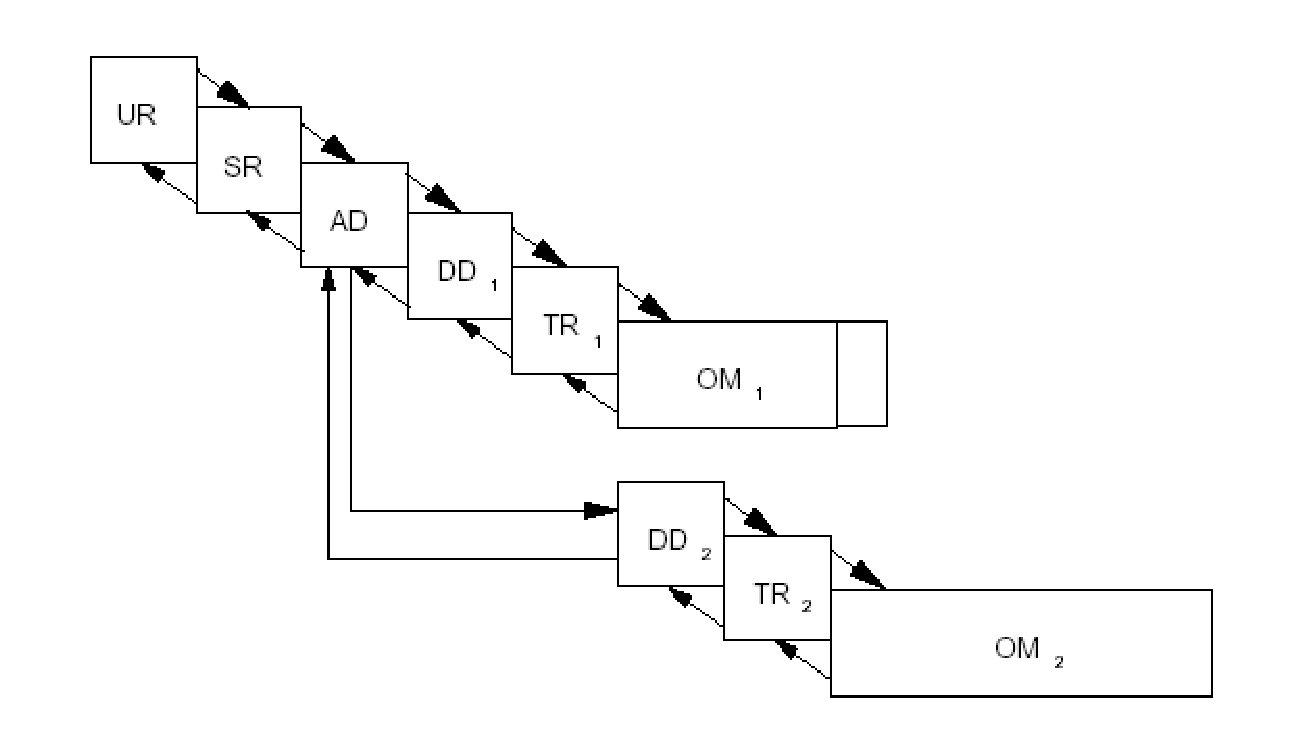
\includegraphics[width=\textwidth]{./figure/incremental_life_cycle.eps}
  \caption{Software life-cycle and input/output documents according to each phase of development.} 
  \label{Fig:Icycle}
\end{figure}

During each increment, software requirements and architectural design documents are reviewed and may be lightly corrected. Detailed design, user manual and testing plans are completed as the work gradually progresses. \\

This life-cycle was chosen for this project because the kernel and basic functionnalities of the platform have to be validated before the development of specific plugins or of a smart interface. \\

\subsubsection{First increment : platform prototype}

This prototype was realised by four students in computer sciences during their final training course. From January to September 2004, they realized a complete increment 
cycle and they considered this first increment as a complete project development from user requirements elicitation to acceptance tests. To reach this objective, they used a standard software life-cycle approach illustrated on figure \ref{Fig:Vcycle}.  
\begin{sidewaysfigure}[hp]
  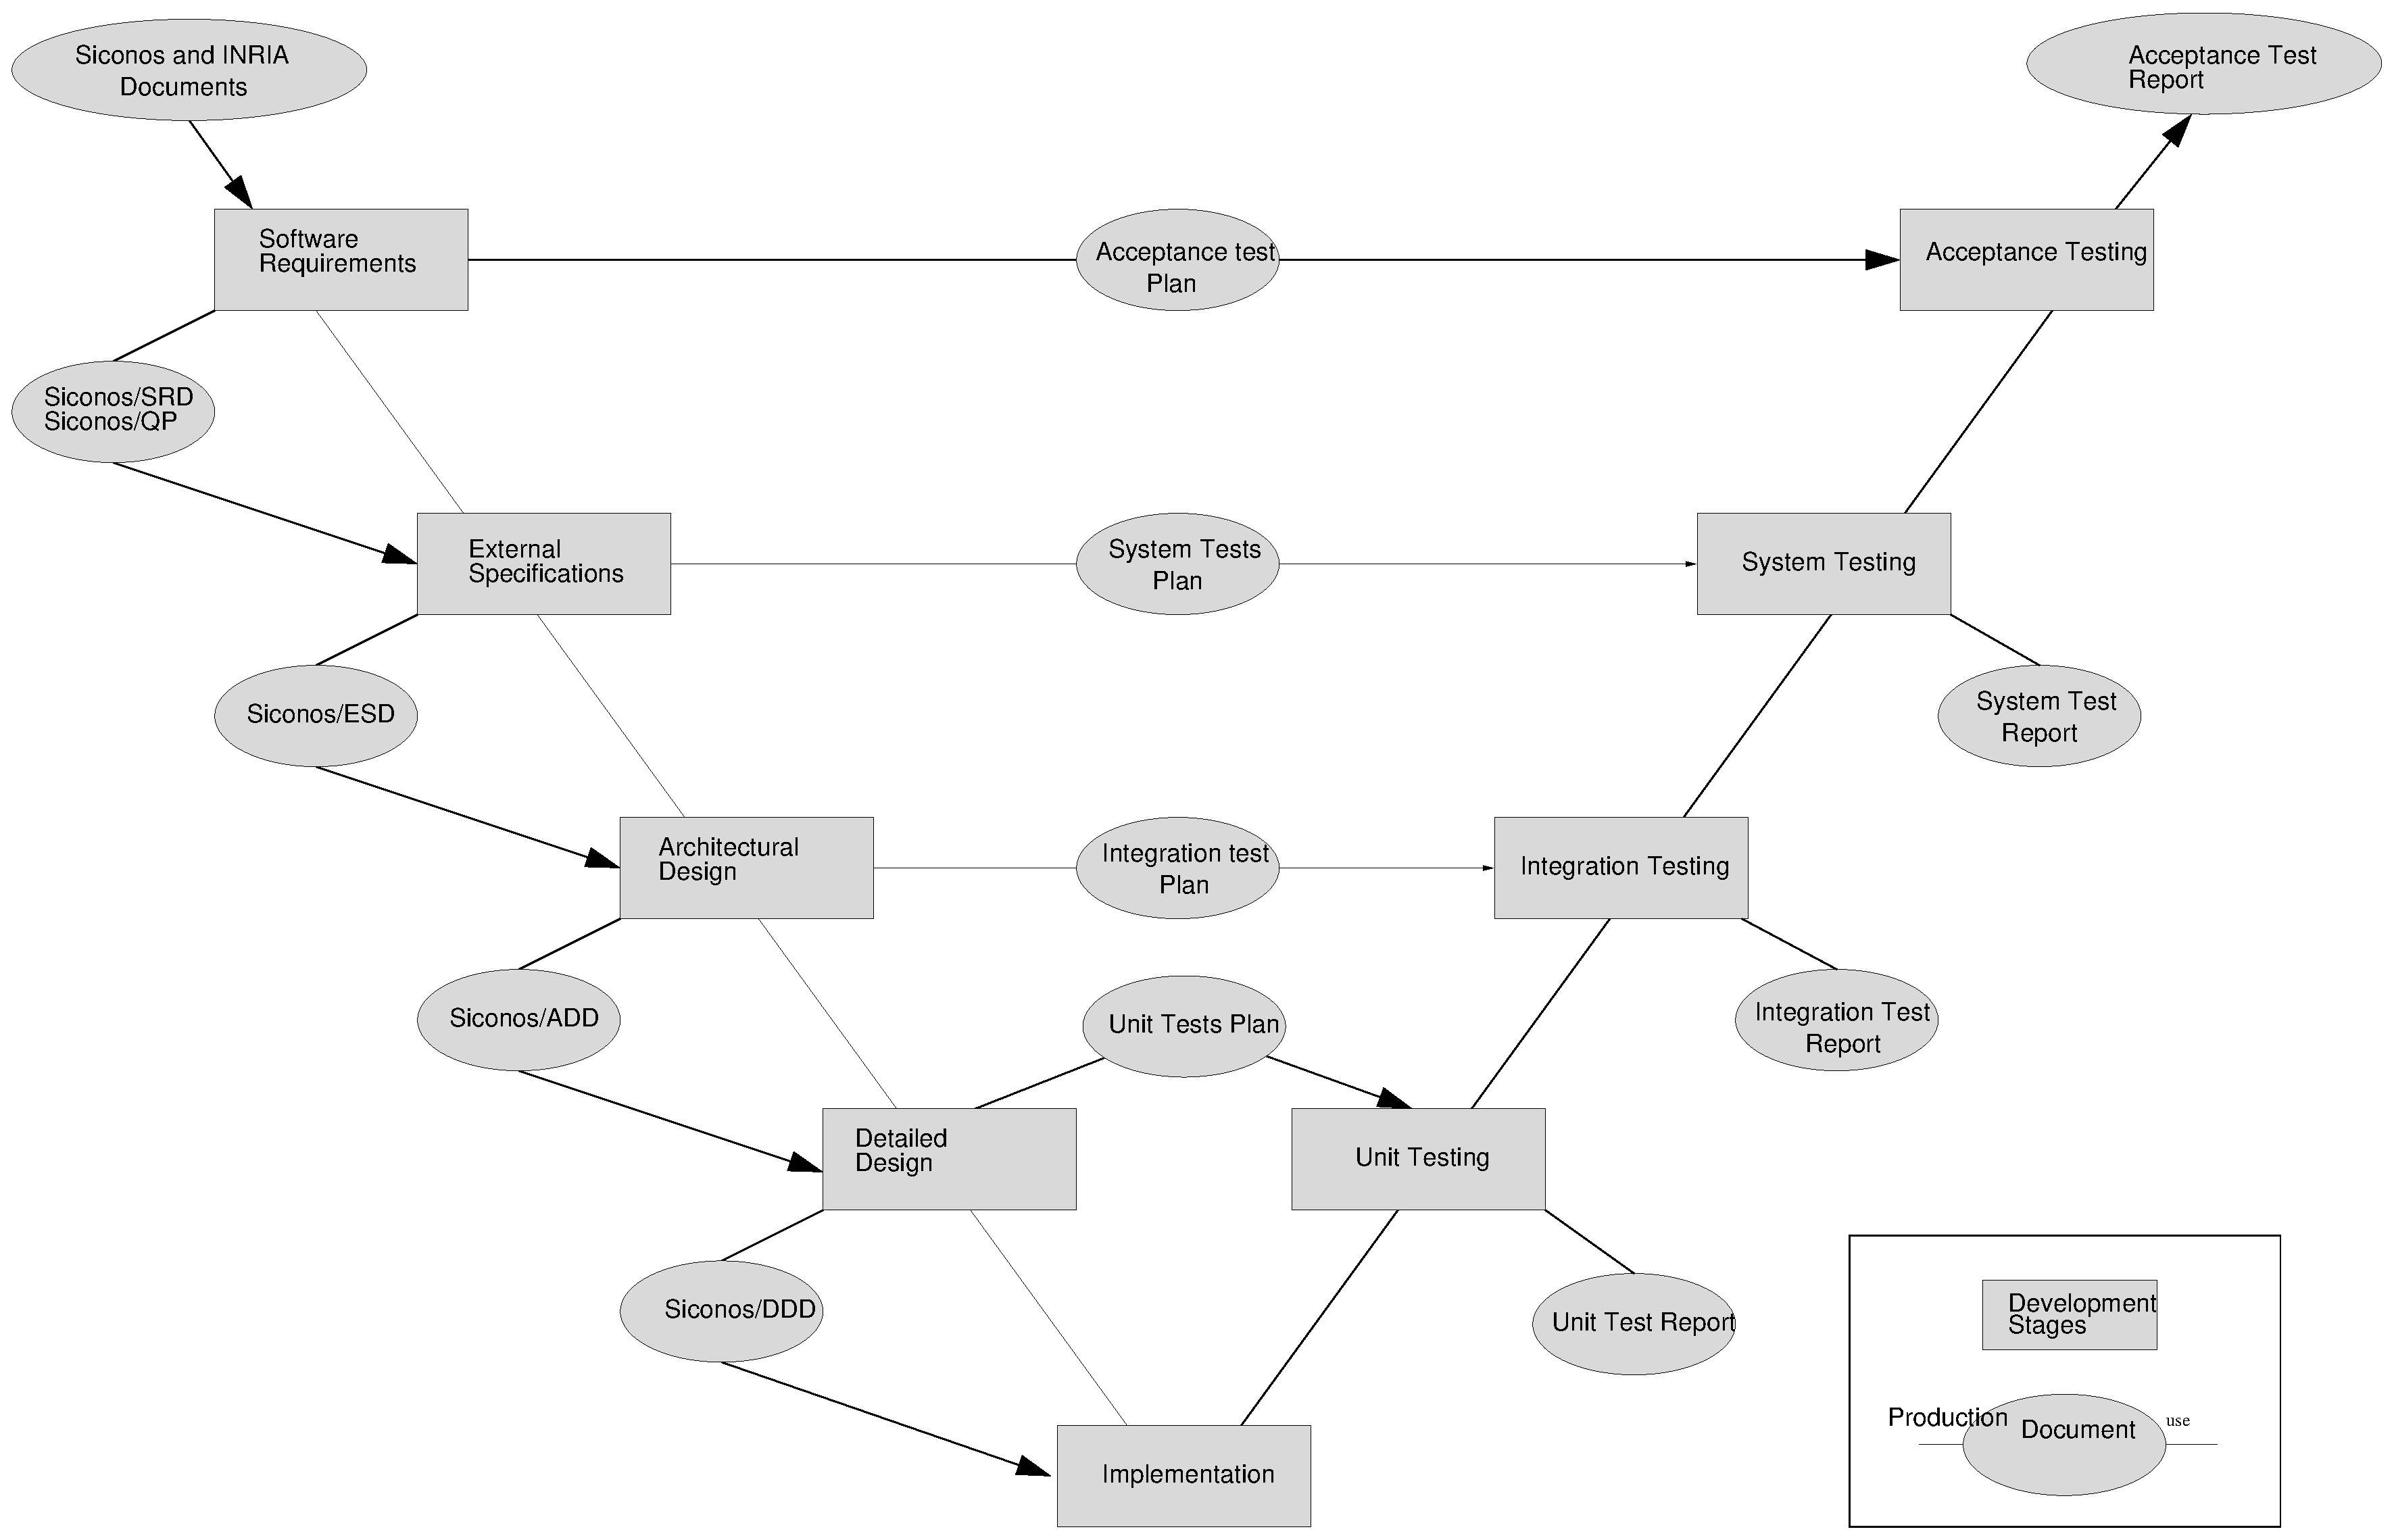
\includegraphics[width=\textwidth]{./figure/Vcycle.eps}
  \caption{Software Life-cycle and input/output documents according to each phase of development.}
  \label{Fig:Vcycle}
\end{sidewaysfigure}

\subsubsection{Development continuation}

The development of the first version of the platform is planned in two others increment, as explained further in this document (see \ref{Subsec:Schedule}).




\subsection{Methods and Models}

\subsubsection{\ac{cocomo}}


This is a cost model for estimating the number of person-months required to develop software. The model also estimates the development schedule in months and produces an effort and schedule distribution by major phases. This model is based on Barry Boehm's ac{cocomo}\footnote{\texttt{http://www1.jsc.nasa.gov/bu2/COCOMO.html}}.Here is what Boehm says about the model: "Basic COCOMO is good for rough order of magnitude estimates of software costs, but its accuracy is necessarily limited because of its lack of factors to account for differences in hardware constraints, personnel quality and experience, use of modern tools and techniques, and other project attributes known to have a significant influence on costs." For more detailed information about \ac{cocomo} and software cost estimating in general, I strongly recommend reading Software Engineering Economics (1981), by Barry Boehm.

The model estimates cost using one of three different development modes: organic, semidetached and embedded. Here is a summary of how Boehm describes the modes:
\begin{itemize}
\item Organic : In the organic mode, relatively small software teams develop software in a highly familiar, in-house environment. 
  Most people connected with the project have extensive experience in working with related systems within the organization, and have a thorough understanding of 
  how the system under development will contribute to the organizations objectives. Very few organic-mode projects have developed products with more than 50 thousand 
  delivered source instructions (KDSI). .
\item Semidetached: The semidetached mode of software development represents an intermediate stage between the organic and embedded modes. "Intermediate" may mean either of two things:
  an intermediate level of project characteristic or a mixture of the organic and embedded mode characteristics.The size range of a semidetached mode product generally 
  extends up to 300 KDSI.
\item Embedded : The major distinguishing factor of an embedded-mode software project is a need to operate within tight constraints. The product must operate within (is embedded in) a strongly coupled complex of hardware, software, regulations, and operational procedures, such as an electronic funds transfer system or an air traffic control system. 
\end{itemize}

\subsubsection{Design method}
\label{Sec:ADD-DesignMethod}


\paragraph{\acs{sd} method.}
The \ac{sd} method is an extension to the \ac{sa} method. This method is based on the analysis of the data flow to get a first level architecture. Then this architecture is evaluated and restructured. This is performed in the seven steps of the method~:

\begin{enumerate}
\item Fundamental diagram
\item Refinement of the data flow diagram
\item Determination of the kind of diagram
\item Plan of the frontier
\item First level architecture
\item Systematic building of the architecture
\item Evaluation and restructuring of the architecture
\end{enumerate}

With this method, one can evaluate the cohesion and the links between modules which is very important for the evolution of the software.
This method will help us to determine the global architecture.
In that way we will be able to design an architecture which will be progressive.
The architecture  must have low links between the different modules and have a high cohesion.

\paragraph{\ac{sd} diagram.}
The \ac{sd} diagram is a data flow diagram. It represents the input and output of informations. It also shows the functions, the data storages and the data flows.

% \paragraph{\acs{uml}}
% The \ac{uml} diagrams are numerous and can modelise lots of relations of the platform to define an adapted architecture to this platform. 

% =====
% UML
% Une architecture adapt�e est la cl� de vo�te du succ�s d'un d�veloppement.
% Elle d�crit des choix strat�giques qui d�terminent en grande partie les qualit�s du logiciel (adaptabilit�,
% performances, fiabilit�...).
% =====


\subsubsection{Models}
\label{Sec:ADD-ModelTool}
To build a good architecture of the platform, we will use various modeling languages and tools. According to the type of information, we want to depict, the  appropriate model to formally represent data, functions, and behaviours of our system. Among them, we can cite the following diagrams :
% \begin{itemize}
% \item \ac{sd} diagram
%   \begin{itemize}
%   \item Data flow diagram\\
%     On this diagram, we represent the input and output of information. We also see the functions, the data storages and the data flows.
%   \end{itemize}



\paragraph{\acs{uml}}
The \ac{uml} diagrams are numerous and can modelise lots of relations of the platform to define an adapted architecture to this platform. 
\begin{itemize}
\item \acs{uml} diagrams.\\
  We will use \ac{uml} tools to create \ac{uml} diagrams.
  With \ac{uml}, we can modelise a big part of the architecture with the numerous \ac{uml} diagrams we will see further, and with \ac{ocl}.

  \begin{itemize}
  \item Sequence diagram\\
    This diagram shows the links of the different actions we can find in the platform.
    It represents the interactions between the entities of the system.

  \item State diagram\\
    This diagram aims to represent automatons as state graphs. It shows the changes of state of an object or a
    module in response to the interactions.

    % ======
    % Ce diagramme sert � repr�senter des automates d'�tats finis, sous forme de graphes d'�tats, reli�s par des arcs 
    % orient�s qui d�crivent les transitions.
    % Les diagrammes d'�tats-transitions permettent de d�crire les changements d'�tats d'un objet ou d'un composant,
    % en r�ponse aux interactions avec d'autres objets/composants ou avec des acteurs.
    % Un �tat se caract�rise par sa dur�e et sa stabilit�, il repr�sente une conjonction instantan�e des valeurs des
    % attributs d'un objet.
    % Une transition repr�sente le passage instantan� d'un �tat vers un autre.
    % ======

  \item Collaboration diagram\\
    This diagram shows the interactions between the objects (instances of classes and actors). It allows to represent
    the context of an interaction.

    % ====
    % Les diagrammes de collaboration montrent des interactions entre objets (instances de classes et acteurs).
    % Ils permettent de repr�senter le contexte d'une interaction, car on peut y pr�ciser les �tats des objets qui 
    % interagissent.
    % ====

  \item Classes diagram\\
    These diagram are collections of classes which show the structure of a model. We use several diagrams for complex models.

    % ====
    % Un diagramme de classes est une collection d'�l�ments de mod�lisation statiques (classes, paquetages...), qui 
    % montre la structure d'un mod�le.
    % Un diagramme de classes fait abstraction des aspects dynamiques et temporels.  
    % Pour un mod�le complexe, plusieurs diagrammes de classes compl�mentaires doivent �tre construits.
    % ====
  \end{itemize}


\item \acs{ocl}\\
  \ac{ocl} is a declarative language for describing rules that apply to UML models developed at IBM and now part of the UML standard.\\
  A formal specification language extension to UML. The Object Constraint Language is a precise text language that provides constraint and object query expressions on an object-oriented model that cannot otherwise be expressed by diagrammatic notation.\\
  OCL supplements UML by providing expressions that have neither the ambiguities of natural language nor the inherent difficulty of using complex mathematics.\\


\end{itemize}



\subsubsection{Format, style and tools for documentation}
All formats, styles and tools for documentation are defined in the \ac{cds}

\subsubsection{Coding standards}


The Coding standards are defined in the \ac{cds}. These standards
will be respected with the help of the Integrated Development
Environment (IDE) Eclipse.


\clearpage

\section{Work Packages, Schedule and Budget}
\label{Sec:QP-PMP-WP}
\begin{ndr}
  To be completed for Analysis and Control
\end{ndr}

\subsection{Work Breakdown Structure}

\paragraph{\ding{85} 1000 Software Project Management}
\begin{itemize}
\item 1100 \ac{numerics} Management
\item 1200 \ac{kernel} Management
\item 1300 \ac{analysis} Management
\item 1400 \ac{control} Management
\item 1500 \ac{imse} Management
\item 1600 Existing softwares and modeling environments review
\item 1700 Relation with other project (Geoplex, Hycon, DaVinci, \dots)
\item 1800 Studying legal aspects  and planning APP deposit
\end{itemize}

\paragraph{\ding{85} 2000 Siconos/Numerics Software Production}
\begin{itemize}
\item 2100 Software Specification phase SSD (Software Requirement and Architectural Design phase) 
  \begin{itemize}
  \item 2110 First Increment Production
    \begin{itemize}
    \item 2111 Global requirements elicitation
      %%% \item 2112 Logical and Physical Model %%%fd je ne comprends pas ce que ca veut dire !!
    \item 2112 Partitionning of the whole requirements into sets of functionalities
    \item 2113 Definition of the priority between sets and of those indispensable
    \item 2114 Definition of some ``minimal'' requirements for a given set 
    \item 2115 Definition of storage method for matrices
    \item 2116 \ac{ssd} draft
    \item 2117 \ac{ssd} final version 
      \begin{itemize}
      \item 2117.1 Global functionalities of the sets
      \item 2117.2 Data input and output
      \item 2117.3 Interface with C++
      \end{itemize}
    \end{itemize}
  \item 2120 Second Increment Production
    \begin{itemize}
    \item 2121 Inclusion of new sets
    \item 2122 SciLab Toolbox
      %% \item 2122 \ac{ssd} final version 
    \end{itemize}
  \item 2130 Third Increment Production
    \begin{itemize}
    \item 2131 Enhancement of included sets
      \begin{itemize}
      \item 2131.1 Adding some specific storage method for matrices 
      \item 2131.2 Adding some specific functionalities
      \item 2131.3 Tuning existing functionnalities for computation performance.   
      \end{itemize}    
    \item 2132 Interface with other langages (Fortran9x, Python, ...)
      %% \item 2134 \ac{ssd} final version 
    \end{itemize}    
  \end{itemize}
  % \item 2200 Architectural Design phase ADD
\item 2200 Detailed Design phase 
  \begin{itemize}
  \item 2210 First Increment Production
    \begin{itemize}
    \item 2211 \ac{dddnumerics} for the first increment sets
      \begin{itemize}
      \item 2211.1 Data Storage descriptions
      \item 2211.2 Detailled interface of functions
      \item 2211.3 Linear Algebra pack 
      \item 2211.4 Solverpack
        
      \end{itemize}

    \item 2212 Interface with C++
    \item 2213 Unit Testing
      \begin{itemize}
      \item 2213.1 Problem samples
      \end{itemize}
    \item 2214 \ac{sumnumerics} for the first increment sets
    \end{itemize}
  \item 2220 Second Increment Production
    \begin{itemize}
    \item 2221  Inclusion of new sets: \ac{ode} pack, root finding
    \item 2222 SciLab Toolbox
    \end{itemize}
  \item 2230 Third Increment Production
    \begin{itemize}
    \item 2231 Sparse storage method for matrices
    \item 2232 Linear Algebra pack for sparse matrices
    \item 2233 Integration of ATLAS
    \item 2234 Block Sparse storage method for matrices
    \item 2235 MPsolver for block sparse  matrices
    \end{itemize}
  \end{itemize}
  % \item 2300 Transfer phase Unit testing
  %   \begin{itemize}
  %   \item 2310 First Increment  Unit testing
  %   \item 2320 Second Increment  Unit testing
  %   \item 2330 Third Increment  Unit testing
  %   \end{itemize}
\item 2300 Transfer phase Acceptance testing
  \begin{itemize}
  \item 2310 First Increment Acceptance testing
    \begin{itemize}
    \item 2311 Acceptance test suite
    \end{itemize}
  \item 2320 Second Increment Acceptance testing
  \item 2330 Third Increment Acceptance testing
  \end{itemize}
\end{itemize}
\paragraph{\ding{85} 3000 Platform kernel~: Siconos/Engine Siconos/Front-End Software Production}
\begin{itemize}
\item 3100 Software Requirements phase  
  \begin{itemize}         
  \item 3110 First Increment Production
    \begin{itemize}         
    \item 3111 Requirements elicitation
    \item 3112 Prototyping and Logical Model
    \item 3113 \ac{srd} draft
    \item 3114 \ac{srd} final 
    \end{itemize}   
  \item 3120 Second Increment Production
    \begin{itemize}         
    \item 3121 Update \ac{srd} according to academical users feedback
    \end{itemize}                   
  \item 3130 Third Increment Production
    \begin{itemize}         
    \item 3131 Update \ac{srd} according to industrial users feedback
    \end{itemize}                   
  \end{itemize}    
\item 3200 External Specification phase
  \begin{itemize}
  \item 3210 First Increment Production
    \begin{itemize}         
    \item 3211 Describing software using context
    \item 3212 Specifying Interfaces
    \item 3213 Input/Output data description
    \item 3214 Error Cases
    \end{itemize}                   
  \item 3220 Second Increment Production
    \begin{itemize}         
    \item 3221 Precising using context and the categories of users.
    \item 3222 Definition and Specification of user interfaces, and tools for their implementation
      \begin{itemize}         
      \item 3222.1 End-user Interface : Scilab interface
      \item 3222.2 Expert-user Interface : Python interface
      \end{itemize}       
    \item 3223 Precise definition for data input/output
      \begin{itemize}         
      \item 3223.1 XML Input/Output
      \item 3223.2 Expert-user Interface for data
      \end{itemize}        
    \end{itemize}   
  \item 3230 Third Increment Production (\ac{tbc})
  \item 3231 Definition of error interface
    \begin{itemize}         
    \item 3231.1 XML database for error messages
    \item 3231.2 Internationalization (?)
    \end{itemize}     
    \begin{itemize}
    \item Linking with existing products
    \end{itemize}
  \end{itemize}
\item 3300 Architectural Design phase
  \begin{itemize}
  \item 3310 First Increment Production
    \begin{itemize}
    \item 3311 Prototyping and Physical Model
    \item 3312 \ac{add} draft
    \item 3313 \ac{add} final
      \begin{itemize}         
      \item 3313.1 SA/SD method application 
      \item 3313.2 Unit descriptions (conceptual class diagrams)
      \item 3313.3 Simulation course (general sequence diagrams)
      \end{itemize}          
    \end{itemize}
  \item 3320 Second Increment Production
    \begin{itemize}         
    \item 3321 Design of user interfaces, and tools for their implementation
      \begin{itemize}         
      \item 3321.1 End-user Interface : Scilab interface
      \item 3321.2 Expert-user Interface : Python interface
      \end{itemize}       
    \item 3322 Design for data input/output
      \begin{itemize}         
      \item 3322.1 XML Input/Output
      \item 3322.2 Expert-user Interface for data
      \end{itemize}        
    \end{itemize}        
  \item 3330 Third Increment Production (\ac{tbc})
    \begin{itemize}
    \item 3331 Design for data input/output
      \begin{itemize}         
      \item 3331.1 End-user Interface for data
      \end{itemize} 
    \end{itemize} 
  \end{itemize}
\item 3400 Detailed Design phase 
  \begin{itemize} 
  \item 3410 First Increment Production
    \begin{itemize}
    \item 3411 \ac{ddd} draft
      \begin{itemize}         
      \item 3411.1 UML Class Diagram
      \item 3411.2 I/O management : XML, "on the fly" nonsmooth dynamical system creation
      \item 3411.3 Software Deliverable Architecture
      \end{itemize}           
    \item 3412 First version of the code
      \begin{itemize}         
      \item 3412.1 Model formalisation Unit
      \item 3412.2 Model strategy Unit
      \item 3412.3 XML I/O Unit
      \item 3412.4 Front-end Unit
      \item 3412.5 Numeric tools Unit
      \end{itemize}           
    \item 3413 Unit Testing
      \begin{itemize}         
      \item 3413.1 CppUnit tests
      \end{itemize}     
    \end{itemize}
  \item 3420 Second Increment Production
    \begin{itemize}
      % \item 3421 Interface Unit Production
      %   \begin{itemize}
      %   \item 3421.1 Plugin system documentation
      %   \item 3421.2 API C
      %   \item 3421.3 Scilab Interface
      %   \item 3421.4 API C++
      %   \item 3421.5 Python Interface
      %   \end{itemize}
    \item 3421 Application Programing Interface
      \begin{itemize}      
      \item 3421.2 Python interface   
      \item 3421.3 Scilab interface   
      \end{itemize}       
    \item 3422 User Interface Unit
      \begin{itemize}      
      \item 3421.1 Scilab interface   
      \item 3421.2 Python interface   
      \end{itemize}                   
    \item 3423 Model Formalisation Unit Production
      % \begin{itemize}
      % \item 3422.1 Adding class of constraints (algebraic bilateral constraints)
      % \item 3422.2 Linear Complemetarity System of relative degree 0 or 1 %Oscillator example
      % \item 3422.3 Lagrangian Non Linear system : plugin Robotics %Robot example
      % \item 3422.4 Relay system %Electrical circuit;
      % \end{itemize}
    \item 3424 Numerical Strategy Unit Production
      % \begin{itemize}
      % \item 3423.1 Event Driven simulation
      % \end{itemize}
    \item 3425 LMGC90 Unit Production
      % \begin{itemize}
      % \item 3424.1 Faisability study with plugin
      % \item 3424.2 \dots
      % \end{itemize}
    \item 3426 XML schema 1.1 compliance
    \end{itemize}
  \item 3430 Third Increment Production \ac{tbd}
  \end{itemize}
\item 3500 Transfer phase
  \begin{itemize} 
  \item 3510 automatic configuration (using Autoconf / Automake)    
  \item 3520 Portability
    \begin{itemize}
    \item 3521 Linux Platform (OS:Red Hat 9, Fedora Core2)
    \item 3522 UNIX Platform (OS:Solaris)
    \item 3523 Windows Platform (OS : Windows 2000/XP, Cygwin environment)  
    \end{itemize}
  \item 3530 Software Transfer Documentation
    \begin{itemize}
    \item 3531 Completing Software User Manual
    \item 3532 Installation documentation
    \end{itemize}
    
  \end{itemize}
\item 3600 Platform Testing
  \begin{itemize} 
  \item 3610 First Increment Testing
    \begin{itemize}
    \item 3611 Templates systems and Benchmark definition
    \item 3612 Integration and system testing
      % \begin{itemize}
      % \item 3611.1 Lagrangian model formalisation
      % \item 3611.2 Time-Stepping strategy
      % \item 3611.3 XML I/O unit               
      % \item 3611.4 Plugin system
      % \end{itemize}
    \item 3613 Acceptance Testing
      % \begin{itemize}
      % \item 3612.1 Bouncing Ball example
      % \end{itemize} 
    \end{itemize}
  \item 3620 Second Increment Testing
    \begin{itemize}
    \item 3621 Templates systems and Benchmark definition
    \item 3622 Integration testing
    \item 3623 System Testing
    \item 3624 Acceptance Testing
      % \begin{itemize}
      % \item 3623.1 Oscillator example
      % \item 3623.2 Robotics example
      % \item 3623.3 Electrical circuit example
      % \end{itemize}  
    \end{itemize}
  \item 3630 Third Increment Testing
    \begin{itemize}
    \item 3631 Templates systems and Benchmark definition (model plugin library)
    \item 3632 Integration testing
    \item 3633 System Testing
    \item 3634 Acceptance Testing    
    \end{itemize}
  \end{itemize}
\end{itemize}
\paragraph{\ding{85} 4000 Siconos/Analysis Software Production \ac{tbd}}
\begin{itemize}
\item 4100 Software Requirements phase SRD 
\item 4200 Architectural Design phase ADD
\item 4300 Detailed Design phase 
\item 4400 Unit testing
\item 4500 Transfer phase Acceptance testing
\end{itemize}
\paragraph{\ding{85} 5000 Siconos/Control Software Production \ac{tbd}}
\begin{itemize}
\item 5100 Software Requirements phase SRD 
\item 5200 Architectural Design phase ADD
\item 5300 Detailed Design phase 
\item 5400 Unit testing
\item 5500 Transfer phase Acceptance testing
\end{itemize}

\paragraph{\ding{85} 6000 Siconos/Pre-Post Software Production \ac{tbd}}
\begin{itemize}
\item 6100 Software Requirements phase SRD 
\item 6200 Architectural Design phase ADD
\item 6300 Detailed Design phase 
\item 6400 Unit testing
\item 6500 Transfer phase Acceptance testing
\end{itemize}

% }


\subsection{Description of the major work packages}

\
In the section above, six  work package has been defined. This first work package, ``\textsf{1000 Software Project Management}'' to the general management of the project. The last three packages are not yet defined in details.



We will   described, in the following  section, the two major work package which are ``\textsf{2000 Siconos/Numerics Software Production}'' and  ``\textsf{3000 Platform kernel Siconos/Engine Siconos/Front-End Software Production }''.

% For each work package, describe the inputs, tasks, outputs, effort requirements, resources allocated and verification process.





\subsubsection{\textsf{2000 Siconos/Numerics Software Production}}



According to the numbering convention of the functionalities in the \ac{srd}, the increments of software production must contain :
\textsf{\begin{itemize}
  \item[2310] First Increment Production\\
    Linear algebra pack : F.1.001; F.1.003.1; F.1.003.2; F.1.010.1;  \\
    MPSolver Pack :  F.1.011.1; F.1.011.2; F.1.011.3; F.1.011.4\\
    C++ interface : F.1.020
  \item[2320] Second Increment Production\\
    ODE Pack : F.1.012;  F.1.013;  F.1.014;\\
    Root finding : F.1.013 \\
    Automatic, analytical and numerical differentiation : F.1.014 \\
    SciLab interface : F.1.020 \\
  \item[2330] Third Increment Production\\
    Linear algebra pack optimisation : F.1.002\\
    Matrices storage methods : F.1.003.4 \\
  \end{itemize}}

This work package is realized by the SICONOS/Numerics defined in the Section \ref{Sec:QP-PMP-PO}. Only S. Nineb, which is a PhD Student hired by the project will work full time for 6 months on this development.  With the other participants, the total resources for this work package may be estimated around 10 man.month. These resources are only sufficient for the design and the development of the first increment. For others increments, it must be planned to hire an other person. 

\subsubsection{\textsf{3000 Platform kernel Siconos/Engine Siconos/Front-End Software Production}}

According to the numbering convention of the functionalities in the \ac{srd}, the increments of software production must contain :
\textsf{  
  \begin{itemize}
  \item[3310] First Increment Production\\    
    API C++ : F.2.000--F.2.002; PER.00 \\
    XML storage files :  F.2.200; F.2.301;    F.2.302;   F.2.304;   DAT.00; F.3.000; INT.00; INT.01;\\
    Basic Plug-in : F.2.042; \\
    Model Formalization : F.2.015; F.2.024; F.2.027; \\
    Numerical strategy : F.2.100;   F.2.102--F.2.105; \\
    Output and Trace values : F.2.303;
  \item[3320] Second Increment Production\\
    API C : F.3.001; \\ 
    Interface between the API C and Scilab \ac{tbd} \\
    Interface between the API C++ and Python \ac{tbd} \\
    Model Formalization  : F.3.001; \\ 
    Numerical strategy : F.2.101; \\
    LMGC90 Plug-in :   F.2.045;
  \item[3330] Third Increment Production\\
    The rest of  functionalities.\ac{tbd}
  \end{itemize}
}

% This work package is the core of the platform. It is realized by Fr�d�ric Dubois, Vincent Acary and four students in software engineering which are hired  for 6 month. The total resources  for this work package is  around 36 man.month. This will be sufficient to carry out the first and the second increments. To carry out the third increment, it is planned to hire a software engineer for the year 2005.
This work package is the core of the platform. It is realized by Fr�d�ric Dubois, Vincent Acary and two software engineers who are hired for 6 month. The total resources  for this work package is  around 36 man.month. This will be sufficient to carry out the first and the second increments. To carry out the third increment, it is planned to hire a software engineer for the year 2005.



\newpage

\subsection{Schedule and milestones}\label{Subsec:Schedule}
\begin{ndr}
  To be completed for Analysis and Control
\end{ndr}
The two following tables present the general planning of SICONOS/WP2.

\begin{longtable}{|l|l|l|}
  \hline
  \rowcolor[gray]{.8}    ID & Milestone & Schedule \\
  \hline
  \hline  
  % \endhead
  \textsf{M1.a} 
  & --- \ac{numerics}: \ac{ssd} draft and MPsolverpack & March 2004 \\
  % &   \textsf{2100; 2200; 2310; 2410}  &  \\
  \hline
  \textsf{M1.b} 
  & --- \ac{srd} and \ac{add} of the kernel draft      &  \\
  % & \textsf{3110; 3120; 3130; 3210; 3220; } & \\ 
  \hline
  \textsf{M2.a} 
  & --- First Increment of the kernel complete (DDD, tests) & June 2004 \\
  % & \textsf{3140; 3230; 3310; 3410;}& \\
  \hline
  \textsf{M2.b} 
  & --- Documentation and Quality reports & September 2004 \\
  % & \textsf{0000;}& \\
  \hline
  \textsf{M3.a} 
  & --- Numerics : first increment complete &  \\
  % & \textsf{0000 }&\\
  & ---            Kernel 1 : API C and C++  &  \\
  % & \textsf{0000 }&\\
  & ---           Kernel 2 : Numerics integration, Numerical and model formalisation  &  \\
  % & \textsf{0000 }&\\
  & ---           Analysis : SRD Draft \ac{tbc} & January 2005 \\
  % & \textsf{4100 }&\\
  \hline
  \textsf{M3.b} 
  & --- Numerics : Second increment complete &  \\
  % & \textsf{0000 }&\\
  & ---           Kernel 1 : Python and Scilab interface, portability &  \\
  % & \textsf{0000}&\\
  & ---           Kernel 2 : coupling LMGC90 to the platform & \\
  % & \textsf{0000}&\\
  & ---           Kernel 3 : First Benchmarks and Demonstation examples &  \\
  % & \textsf{0000}&\\
  & ---            Analysis : \ac{tbd} & March 2005 \\
  % & \textsf{0000}&\\
  \hline
  \textsf{M4.a} 
  & --- Third Increment of kernel (model and numerical formalization) &  \\
  % & \textsf{3320; 3420 }&\\
  & ---            Model Plugin Library (Benchmarks and Demonstation examples)  &  \\
  % & \textsf{0000 }&\\
  & ---           Analysis : development complete \ac{tbc}   & June 2005  \\
  % & \textsf{4300; 4400; 4500 }&\\
  \hline
  \textsf{M4.b} 
  
  & --- Numerics : Third increment complete   & September 2005 \\ 
  & --- Kernel : First distribution version with Scilab and Python Interfaces    &  \\
  % &  \textsf{0000}&\\
  \hline
  \textsf{M5} 
  & ---    First increment of \ac{control} complete \ac{tbc} & March 2006 \\
  % & \textsf{5000}&\\   
  \hline
  \textsf{M6} 
  & ---    Implementation of the \ac{imse} complete \ac{tbc} & September 2006 \\
  % & \textsf{6000}&\\    
  \hline
  \caption{Definition of Milestones}
  \label{Tab:milestones}
\end{longtable}
\newpage

\begin{landscape}
  % %% LyX 1.3 created this file.  For more info, see http://www.lyx.org/.
% %% Do not edit unless you really know what you are doing.
% \documentclass[a4paper,landscape,english]{extarticle}
% \usepackage[T1]{fontenc}
% \usepackage[latin1]{inputenc}
% \usepackage{array}
% \usepackage{longtable}

% \makeatletter

% %%%%%%%%%%%%%%%%%%%%%%%%%%%%%% LyX specific LaTeX commands.
% %% Because html converters don't know tabularnewline
% \providecommand{\tabularnewline}{\\}

% \usepackage{babel}
% \makeatother
% \begin{document}
\renewcommand{\arraystretch}{0.8}
\begin{longtable}{|l||l||c|c||c|c||c|c||c|c||c|c||c|c||}
\hline 
&
&
\multicolumn{12}{c|}{{\scriptsize Milestones}}\tabularnewline
\hline 
&
{\scriptsize Milestone title}&
\multicolumn{2}{c||}{\scriptsize M1}&
\multicolumn{2}{c||}{\scriptsize M2}&
\multicolumn{2}{c||}{\scriptsize M3}&
\multicolumn{2}{c||}{\scriptsize M4}&
\multicolumn{2}{c||}{\scriptsize M5}&
\multicolumn{2}{c||}{\scriptsize M6}
\tabularnewline
\hline
&
{\scriptsize Years}&
&
\multicolumn{4}{c|}{\scriptsize 2004}&
\multicolumn{4}{c|}{\scriptsize 2005}&
\multicolumn{3}{c|}{\scriptsize 2006}
\tabularnewline
\hline 
{\scriptsize Task Number}&
{\scriptsize Task title............................................................Quarters
(from September 2003)}&
{\scriptsize 01}&
{\scriptsize 02}&
{\scriptsize 03}&
{\scriptsize 04}&
{\scriptsize 05}&
{\scriptsize 06}&
{\scriptsize 07}&
{\scriptsize 08}&
{\scriptsize 09}&
{\scriptsize 10}&
{\scriptsize 11}&
{\scriptsize 12}\tabularnewline
\endhead
\hline 
&
&
\multicolumn{12}{c|}{{\scriptsize Milestones}}\tabularnewline
\hline 
&
{\scriptsize Milestone title}&
\multicolumn{2}{c||}{\scriptsize M1}&
\multicolumn{2}{c||}{\scriptsize M2}&
\multicolumn{2}{c||}{\scriptsize M3}&
\multicolumn{2}{c||}{\scriptsize M4}&
\multicolumn{2}{c||}{\scriptsize M5}&
\multicolumn{2}{c||}{\scriptsize M6}
\tabularnewline
\hline
&
{\scriptsize Years}&
&
\multicolumn{4}{c|}{\scriptsize 2004}&
\multicolumn{4}{c|}{\scriptsize 2005}&
\multicolumn{3}{c|}{\scriptsize 2006}
\tabularnewline
\hline 
{\scriptsize Task Number}&
{\scriptsize Task title............................................................Quarters
(from September 2003)}&
{\scriptsize 01}&
{\scriptsize 02}&
{\scriptsize 03}&
{\scriptsize 04}&
{\scriptsize 05}&
{\scriptsize 06}&
{\scriptsize 07}&
{\scriptsize 08}&
{\scriptsize 09}&
{\scriptsize 10}&
{\scriptsize 11}&
{\scriptsize 12}
\tabularnewline
\endfirsthead
\hline 
\multicolumn{14}{|c|}{\textbf{\scriptsize Software Project Management}}\tabularnewline
\hline 
{\scriptsize 1100}&
{\scriptsize Existing softwares and modeling environments review }&
&
&
&
&
&
&
&
&
&
&
&
\tabularnewline
\hline 
{\scriptsize 1200}&
{\scriptsize Relation with other projects (Hycon, DaVinci) }&
&
&
&
&
&
&
&
&
&
&
&
\tabularnewline
\hline 
{\scriptsize 1300}&
{\scriptsize Studying legal aspects and planing APP deposit}&
&
&
&
&
&
&
{\footnotesize X}&
&
&
&
&
\tabularnewline
\hline 
\pagebreak
\multicolumn{14}{|c|}{\textbf{\scriptsize Siconos/Numerics Software Production}}
\tabularnewline
\hline 
{\scriptsize 2110}&
{\scriptsize Software Specification and architectural design phase - First increment}&
&
&
&
&
{\footnotesize X} &
&
&
&
&
&
&
\tabularnewline
\hline
{\scriptsize 2120}&
{\scriptsize Software Specification and architectural design phase - Second increment}&
&
&
&
&
&
{\footnotesize X} &
&
&
&
&
&
\tabularnewline
\hline
{\scriptsize 2130}&
{\scriptsize Software Specification and architectural design phase - Third increment}&
&
&
&
&
&
&
&
{\footnotesize X} &
&
&
&
\tabularnewline
\hline 
{\scriptsize 2210}&
{\scriptsize First Increment Production}&
&
&
&
&
{\footnotesize X} &
&
&
&
&
&
&
\tabularnewline
\hline 
{\scriptsize 2220}&
{\scriptsize Second Increment Production}&
&
&
&
&
&
{\footnotesize X} &
&
&
&
&
&
\tabularnewline
\hline 
{\scriptsize 2230}&
{\scriptsize Third Increment Production}&
&
&
&
&
&
&
&
{\footnotesize X} &
&
&
&
\tabularnewline
\hline 
{\scriptsize 2310}&
{\scriptsize Transfer phase Acceptance testing - First increment}&
&
&
&
&
{\footnotesize X} &
&
&
&
&
&
&
\tabularnewline
\hline 
{\scriptsize 2320}&
{\scriptsize Transfer phase Acceptance testing - Second increment }&
&
&
&
&
&
{\footnotesize X} &
&
&
&
&
&
\tabularnewline
\hline 
{\scriptsize 2330}&
{\scriptsize Transfer phase Acceptance testing - Third increment }&
&
&
&
&
&
&
&
{\footnotesize X} &
&
&
&
\tabularnewline
\hline 
\multicolumn{14}{|c|}{\textbf{\scriptsize Platform kernel : Siconos/Engine Siconos/Front-End
Software Production}}\tabularnewline
\hline 
{\scriptsize 3110}&
{\scriptsize Requirements elicitation}&
{\footnotesize X}&
&
&
&
&
&
&
&
&
&
&
\tabularnewline
\hline 
{\scriptsize 3120}&
{\scriptsize SRD Revision - Second increment}&
&
&
&
&
{\footnotesize X}&
&
&
&
&
&
&
\tabularnewline
\hline 
{\scriptsize 3130}&
{\scriptsize SRD Revison - third increment}&
&
&
&
&
&
&
{\footnotesize X}&
&
&
&
&
\tabularnewline
\hline 
{\scriptsize 3210}&
{\scriptsize External Specifications Phase - first increment}&
&
{\footnotesize X}&
&
&
&
&
&
&
&
&
&
\tabularnewline
\hline 
{\scriptsize 3220}&
{\scriptsize External Specifications Phase - second increment}&
&
&
&
&
&
{\footnotesize X}&
&
&
&
&
&
\tabularnewline
\hline 
{\scriptsize 3230}&
{\scriptsize External Specifications Phase - third increment}&
&
&
&
&
&
&
{\footnotesize X}&
&
&
&
&
\tabularnewline
\hline 
{\scriptsize 3310}&
{\scriptsize Architectural Design - first increment}&
&
&
{\footnotesize X}&
&
&
&
&
&
&
&
&
\tabularnewline
\hline 
{\scriptsize 3320}&
{\scriptsize Architectural Design - second increment }&
&
&
&
&
&
{\footnotesize X}&
&
&
&
&
&
\tabularnewline
\hline 
{\scriptsize 3330}&
{\scriptsize Architectural Design - third increment}&
&
&
&
&
&
&
{\footnotesize X}&
&
&
&
&
\tabularnewline
\hline 
{\scriptsize 3410}&
{\scriptsize Detail Design and coding - first increment}&
&
&
&
{\footnotesize X}&
&
&
&
&
&
&
&
\tabularnewline
\hline
{\scriptsize 3420}&
{\scriptsize Detail Design and coding - second increment}&
&
&
&
&
&
&
{\footnotesize X}&
&
&
&
&
\tabularnewline
\hline
{\scriptsize 3430}&
{\scriptsize Detail Design and coding - third increment}&
&
&
&
&
&
&
&
{\footnotesize X}&
&
&
&
\tabularnewline
\hline 
{\scriptsize 3510}&
{\scriptsize Platform Testing - first increment}&
&
&
&
{\footnotesize X}&
&
&
&
&
&
&
&
\tabularnewline
\hline 
{\scriptsize 3520}&
{\scriptsize Platform Testing - second increment}&
&
&
&
&
&
&
{\footnotesize X}&
&
&
&
&
\tabularnewline
\hline 
{\scriptsize 3530}&
{\scriptsize Platform Testing - third increment}&
&
&
&
&
&
&
&
{\footnotesize X}&
&
&
&
\tabularnewline
\hline
{\scriptsize 3610}&
{\scriptsize Transfer Phase - Automatic configuration}&
&
&
&
&
{\footnotesize X}&
&
&
&
&
&
&
\tabularnewline
\hline 
{\scriptsize 3620}&
{\scriptsize Transfer Phase - Portability}&
&
&
&
&
&
{\footnotesize X}&
&
&
&
&
&
\tabularnewline
\hline 
{\scriptsize 3630}&
{\scriptsize Transfer Phase - Software installation and using documentation}&
&
&
&
&
&
{\footnotesize X}&
&
&
&
&
&
\tabularnewline
\hline  
\multicolumn{14}{|c|}{\textbf{\scriptsize Siconos/Analysis Software Production}}
\tabularnewline
\hline 
{\scriptsize 4100}&
{\scriptsize Siconos/Analysis Software Requirements}&
&
&
&
&
&
{\footnotesize X}&
&
&
&
&
&
\tabularnewline
\hline
{\scriptsize 4200}&
{\scriptsize Siconos/Analysis Architectural Design}&
&
&
&
&
&
&
{\footnotesize X}&
&
&
&
&
\tabularnewline
\hline
{\scriptsize 4300}&
{\scriptsize Siconos/Analysis Detailed Design}&
&
&
&
&
&
&
{\footnotesize X}&
&
&
&
&
\tabularnewline
\hline
{\scriptsize 4400}&
{\scriptsize Siconos/Analysis Unit Testing}&
&
&
&
&
&
&
{\footnotesize X}&
&
&
&
&
\tabularnewline
\hline
{\scriptsize 4500}&
{\scriptsize Siconos/Analysis Acceptance Testing}&
&
&
&
&
&
&
{\footnotesize X}&
&
&
&
&
\tabularnewline
\hline
\multicolumn{14}{|c|}{\textbf{\scriptsize Siconos/Control Software Production}}\tabularnewline
\hline 
{\scriptsize 5100}&
{\scriptsize Siconos/Control Software Requirements}&
&
&
&
&
&
&
&
&
&
{\footnotesize X}&
&
\tabularnewline
\hline
{\scriptsize 5200}&
{\scriptsize Siconos/Control Architectural Design}&
&
&
&
&
&
&
&
&
&
{\footnotesize X}&
&
\tabularnewline
\hline
{\scriptsize 5300}&
{\scriptsize Siconos/Control Detailed Design}&
&
&
&
&
&
&
&
&
&
&
{\footnotesize X}&
\tabularnewline
\hline
{\scriptsize 5400}&
{\scriptsize Siconos/Control Unit Testing}&
&
&
&
&
&
&
&
&
&
&
{\footnotesize X}&
\tabularnewline
\hline
{\scriptsize 5500}&
{\scriptsize Siconos/Control Acceptance Testing}&
&
&
&
&
&
&
&
&
&
&
{\footnotesize X}&
\tabularnewline
\hline
\multicolumn{14}{|c|}{\textbf{\scriptsize Siconos/Pre/Post Software Production}}\tabularnewline
\hline 
{\scriptsize 6100}&
{\scriptsize Siconos/Pre/Post Software Requirements}&
&
&
&
&
&
&
&
&
&
&
&
{\footnotesize X}
\tabularnewline
\hline
{\scriptsize 6200}&
{\scriptsize Siconos/Pre/Post Architectural Design}&
&
&
&
&
&
&
&
&
&
&
&
{\footnotesize X}
\tabularnewline
\hline
{\scriptsize 6300}&
{\scriptsize Siconos/Pre/Post Detailed Design}&
&
&
&
&
&
&
&
&
&
&
&
{\footnotesize X}
\tabularnewline
\hline
{\scriptsize 6400}&
{\scriptsize Siconos/Pre/Post Unit Testing}&
&
&
&
&
&
&
&
&
&
&
&
{\footnotesize X}
\tabularnewline
\hline
{\scriptsize 6500}&
{\scriptsize Siconos/Pre/Post Acceptance Testing}&
&
&
&
&
&
&
&
&
&
&
&
{\footnotesize X}
\tabularnewline
\hline
\caption{Relation between Work Breakdowm Structure and Milestones}
\label{Tab:WBS and milestones}
\end{longtable}
%\end{document}

\end{landscape}



\subsection{Details on Organisational roles and responsibilities}
\label{Sec:Roles}
\begin{ndr}
  To be completed for Analysis and Control
\end{ndr}


We give in this section more details on the role and the responsabilities of each Team with the respect to the Work Breakdown structure and the Milestones.
To get  more details about developments teams, see \ref{Sec:QP-PMP-PO}.\\

\begin{landscape}
  \renewcommand{\arraystretch}{0.95}
\begin{longtable}{|l|l|l|l|}
  \hline
  \rowcolor[gray]{.8} Team & Task Responsible & Task Number and Title & Milest. \\
  \hline
  \endhead
  \multicolumn{4}{|c|}{\textbf{\scriptsize Software Project Management}}\\
  \hline 
  INRIA & FD &   1100 \ac{numerics} Management       & -- \\ \hline
  INRIA & VA &   1200 \ac{kernel} Management      & -- \\ \hline
  INRIA & PP &   1300 \ac{analysis} Management    & -- \\ \hline
  INRIA & \ac{tbd}  &   1400 \ac{control} Management       & -- \\ \hline
  INRIA & \ac{tbd}  &   1500  \ac{imse} Management     & -- \\ \hline
  INRIA & VA &   1600 Existing softwares and modeling environments review       & M3.a \\ \hline
  INRIA & VA &   1700 Relation with other project (Hycon, DaVinci,\dots)        & M3.a \\ \hline
  INRIA & VA,FD &   1800 Studying legal aspect and planning APP deposit    & M4.a \\ \hline
  \pagebreak
  \multicolumn{4}{|c|}{\textbf{\scriptsize Siconos/Numerics Software Production}} \\  \hline  
  LMGC & FD &   2100 Software Specification phase SSD   & MIST \\ \hline
  LMGC & FD &   2110 First Increment Production         & M3.a \\ \hline
  LMGC & FD &   2111 Global requirements elicitation    & M3.a \\ \hline
  LMGC & FD &   2112 Partitionning of the whole requirements into sets of functionnalities      & M3.a \\ \hline
  LMGC & FD &   2113 Definition of the priority between sets (essential sets)                   & M3.a \\ \hline
  LMGC & FD &   2114 Definition of some "minimal" requirements for a given set                  & M3.a \\ \hline
  LMGC & FD &   2115 Definition of storage method for matrices  & M3.a \\ \hline
  LMGC & FD &   2116 \ac{ssd} draft                             & M3.a \\ \hline
  LMGC & FD &   2117 \ac{ssd} final                     & M3.a \\ \hline
  LMGC & FD &   2117.1 Functions of the software & M3.a \\ \hline
  LMGC & FD &   2117.2 Data input and output    & M3.a \\ \hline
  LMGC & FD &   2117.3 Interface with C++               & M3.a \\ \hline
  LMGC & FD &   2120 Second Increment Production        & M3.b \\ \hline
  LMGC & FD &   2121 Inclusion of new sets              & M3.b \\ \hline
  LMGC & FD &   2122 SciLab toolbox			            & M3.b \\ \hline
  LMGC & FD &   2130 Third Increment Production         & M4.b \\ \hline
  LMGC & FD &   2131 Enhancement of included sets       & M4.b \\ \hline
  LMGC & FD &   2131.1 Adding some specific storage method for matrices & M4.b \\ \hline
  LMGC & FD &   2131.2 Adding some specific functionalities                         & M4.b \\ \hline
  LMGC & FD &   2131.3 Tuning existing functionnalities for computation performance & M4.b \\ \hline
  LMGC & FD &   2132 Interface with other langages (Fortran9x, Python, ...)     & M4.b \\ \hline
  LMGC & FD &   2200 Detailed Design phase              & M3.a \\ \hline
  LMGC & FD &   2210 First Increment Production         & M3.a \\ \hline
  LMGC & FD &   2211 \ac{dddnumerics}                   & M3.a \\ \hline
  LMGC & FD &   2211.1 Data Storage descriptions        & M3.a \\ \hline
  LMGC & FD &   2211.2 Detailled interface of functions & M3.a \\ \hline
  LMGC & FD &   2211.3 Linear Algebra pack              & M3.a \\ \hline
  LMGC & FD &   2211.4 Solverpack                       & M3.a \\ \hline
  LMGC & FD &   2212 Interface with C++                 & M3.a \\ \hline
  LMGC & FD &   2213 Unit Testing                       & M3.a \\ \hline
  LMGC & FD &   2213.1 Problem samples          & M3.a \\ \hline
  LMGC & FD &   2214 \ac{sumnumerics}           & M3.a \\ \hline
  LMGC & FD &   2220 Second Increment Production        & M3.b \\ \hline
  LMGC & FD &   2221 Inclusion of new sets \ac{ode} pack& M3.b \\ \hline
  LMGC & FD &   2222 SciLab toolbox				        & M3.b \\ \hline
  LMGC & FD &   2230 Third Increment Production         & M4.b \\ \hline
  LMGC & FD &   2231 Sparse storage method for matrices & M4.b \\ \hline
  LMGC & FD &   2232 Linear Algebra pack for sparse matrices& M4.b \\ \hline
  LMGC & FD &   2233 Integration of \ac{atlas}		    & M4.b \\ \hline
  LMGC & FD &   2234 Block sparse storage method for matrices& M4.b \\ \hline
  LMGC & FD &   2235 MPSolver for block sparse matrices & M4.b \\ \hline
  LMGC & FD &   2300 Transfer phase Acceptance testing  & M3.a \\ \hline
  LMGC & FD &   2310 First Increment Acceptance testing & M3.a \\ \hline
  LMGC & FD &   2311 Acceptance test suite              & M3.a \\ \hline
  LMGC & FD &   2320 Second Increment Acceptance testing& M3.b \\ \hline
  LMGC & FD &   2330 Third Increment Acceptance testing & M4.b \\ \hline

  
\pagebreak
\multicolumn{4}{|c|}{\textbf{\scriptsize Platform kernel : Siconos/Engine Siconos/Front-End Software Production}}\\ \hline 
  INRIA, LMGC & VA, FD, JB, JMB &   3100 Software Requirements phase   &  \\ \hline
  INRIA, LMGC & VA, FD, JB, JMB &   3110 First Increment Production  & M1.b \\ \hline
  INRIA, LMGC & VA, FD &   3111 Requirements elicitation                & M1.a \\ \hline
  INRIA, LMGC & VA, FD &   3112 Prototyping and Logical Model   & M1.a \\ \hline
  INRIA, LMGC & VA, FD &   3113 \ac{srd} draft          & M1.a \\ \hline
  INRIA & VA, JBC, JMB &   3114 \ac{srd} final          & M1.b \\ \hline
  INRIA, LMGC & VA, FD &   3120 Second Increment Production     & M3.a \\ \hline
  INRIA, LMGC & VA, FD &   3121 Update \ac{srd} according to academical users feedback  & M3.a \\ \hline
  INRIA, LMGC & VA, FD &   3130 Third Increment Production      & M4.a \\ \hline
  INRIA, LMGC & VA, FD &   3131 Update \ac{srd} according to industrial users feedback  & M4.a \\ \hline
  INRIA & VA, JBC, JMB &   3200 External Specification phase    &  \\ \hline
  INRIA & VA, JBC, JMB &   3210 First Increment Production              & M1.b \\ \hline
  INRIA & VA, JBC, JMB &   3211 Describing software using context & M1.b \\ \hline
  INRIA & VA, JBC, JMB &   3212 Specifying Interfaces                   & M1.b \\ \hline
  INRIA & VA, JBC, JMB &   3213 Input/Output data description   & M1.b \\ \hline
  INRIA & VA, JBC, JMB &   3214 Error Cases             & M1.b \\ \hline
  INRIA, LMGC & JBC, JMB &   3220 Second Increment Production   & M3.b \\ \hline
  INRIA & JBC &   3221 Precising using context and the categories of users. & M3.b \\ \hline
  INRIA & JBC &   3222 Definition and Specification of user interfaces, and tools  & M3.b \\ \hline
  INRIA & JBC &   3222.1 End-user Interface : Scilab interface & M3.b \\ \hline
  INRIA & JBC &   3222.2 Expert-user Interface : Python interface & M3.b \\ \hline
  LMGC & JMB &   3223 Precise definition for data input/output  & M3.b \\ \hline
  LMGC & JMB &  3223.1 XML Input/Output & M3.b \\ \hline
  LMGC & JMB &  3223.2 Expert-user Interface for data & M3.b \\ \hline
  LMGC & JMB &   3224 Definition of error interface                     & M3.b \\ \hline
  INRIA, LMGC & VA, FD &   3230 Third Increment Production - Linking with existing products  & M4.a \\ \hline
  INRIA & VA, JBC, JMB &   3300 Architectural Design phase      &  \\ \hline
  INRIA & VA, JBC, JMB &   3310 First Increment Production      & M2.a \\ \hline
  INRIA & VA, JBC, JMB &   3311 Prototyping and Physical Model  & M2.a \\ \hline
  INRIA & VA, JBC, JMB &   3312 \ac{add} draft          & M2.a \\ \hline
  INRIA & JMB &   3313 \ac{add} final  & M2.a \\ \hline
  INRIA & JMB &   3313.1 SA/SD method application  & M2.a \\ \hline
  INRIA & JMB &   3313.2 Unit descriptions (conceptual class diagrams)  & M2.a \\ \hline
  INRIA & JMB &   3313.3 Simulation course (general sequence diagrams)  & M2.a \\ \hline
  INRIA, LMGC &  VA, FD, JB, JMB &   3320 Second Increment Production   & M3.b \\ \hline
  INRIA & JBC &  3321 Design of user interfaces, and tools for their implementation & M3.b \\ \hline        
  INRIA & JBC &  3321.1 End-user Interface : Scilab interface   & M3.b \\ \hline
  INRIA & JBC &  3321.2 Expert-user Interface : Python interface  & M3.b \\ \hline
  LMGC & JMB & 3322 Design for data input/output & M3.b \\ \hline       
  LMGC & JMB & 3322.1 XML Input/Output & M3.b \\ \hline
  LMGC & JMB & 3322.2 Expert-user Interface for data & M3.b \\ \hline
  INRIA, LMGC &  VA, FD &   3330 Third Increment Production    & M4.a \\ \hline
  INRIA, LMGC &  VA, FD & 3331 Design for data input/output  & M4.a \\ \hline        
  INRIA, LMGC &  VA, FD & 3331.1 End-user Interface for data  & M4.a \\ \hline
  INRIA, LMGC & VA, FD, JB, JMB &   3400 Detailed Design phase                  &  \\ \hline
  INRIA & VA, JBC, JMB &   3410 First Increment Production                      & M2.b \\ \hline
  INRIA & VA, JBC, JMB &   3411 \ac{ddd} draft          & M2.b \\ \hline
  INRIA & JMB &   3411.1 UML Class Diagram                      & M2.b \\ \hline
  INRIA & JMB &   3411.2 I/O management : XML, "on the fly" dynamical system creation & M2.b \\ \hline
  INRIA & JBC &   3411.3 Software Deliverable Architecture  & M2.b \\ \hline
  INRIA & VA, JBC, JMB &   3412 First version of the code       & M2.b \\ \hline
  INRIA & VA, JBC, JMB &   3412.1 Model formalisation Unit      & M2.b \\ \hline
  INRIA & VA, JBC, JMB &   3412.2 Model strategy Unit   & M2.b \\ \hline
  INRIA & JMB &   3412.3 XML I/O Unit                                   & M2.b \\ \hline
  INRIA & VA, JBC, JMB &   3412.4 Front-end Unit                & M2.b \\ \hline
  INRIA & JBC &   3412.5 Numeric tools Unit                     & M2.b \\ \hline
  INRIA, LMGC & JBC, JMB &   3413 Unit Testing                  & M2.b \\ \hline
  INRIA & JBC, JMB &   3413.1 CppUnit tests                     & M2.b \\ \hline
  INRIA, LMGC & VA, FD, JBC, JMB &   3420 Second Increment Production  & M3.b \\ \hline
  INRIA & JBC &   3421 Application Programing Interface  & M3.b \\ \hline
  INRIA & JBC &   3421.2 Python interface                       & M3.b \\ \hline
  INRIA & JBC &   3421.3 Scilab interface                               & M3.b \\ \hline
  INRIA & JBC &   3422 User Interface Unit              & M3.b \\ \hline
  INRIA & JBC &   3421.1 Scilab interface               & M3.b \\ \hline
  INRIA & JBC &   3421.2 PythonScilab interface         & M3.b \\ \hline
  INRIA, LMGC & VA, FD, JMB &   3423 Model Formalisation Unit Production  & M4.a \\ \hline
  INRIA, LMGC & VA, FD, JMB &   3424 Numerical Strategy Unit Production  & M4.a \\ \hline
  LMGC & FD, JMB &   3425 LMGC'90 Unit Production               & M4.a \\ \hline
  LMGC & JMB &   3426 XML schema 1.1 compliance                 & M3.b \\ \hline
  INRIA, LMGC & VA, FD &   3430 Third Increment Production  & M4.b \\ \hline 
  INRIA, LMGC & VA, FD, JBC, JMB &   3500 Platform Testing  &  \\ \hline
  INRIA & JBC, JMB &   3510 First Increment Testing                     & M2.b \\ \hline
  INRIA & VA &   3511 Templates systems and Benchmark definition & M2.a \\ \hline
  INRIA & JBC, JMB &   3512 Integration and system testing      & M2.b \\ \hline
  INRIA & VA, JBC, JMB &   3513 Acceptance Testing                      & M2.b \\ \hline
  INRIA, LMGC & JBC, JMB &   3520 Second Increment Testing      & M4.a \\ \hline
  INRIA, LMGC & VA, FD, JBC, JMB &   3521 Templates systems and Benchmark definition & M4.a \\ \hline
  INRIA, LMGC & JBC, JMB &   3522 Integration testing                   & M4.a \\ \hline
  INRIA, LMGC & JBC, JMB &   3523 System Testing                                & M4.a \\ \hline
  INRIA, LMGC & VA, FB, JBC, JMB &   3524 Acceptance Testing    & M4.a \\ \hline
  INRIA, LMGC & VA, FD &   3530 Third Increment Testing                 & M4.b \\ \hline
  INRIA, LMGC & VA, FD &   3531 Templates systems and Benchmark definition (model plugin library) & M4.b \\ \hline
  INRIA, LMGC & VA, FD &   3532 Integration testing             & M4.b \\ \hline
  INRIA, LMGC & VA, FD &   3533 System Testing                          & M4.b \\ \hline
  INRIA, LMGC & VA, FD &   3534 Acceptance Testing              & M4.b \\ \hline
  INRIA, LMGC & JBC, JMB &   3600 Transfer phase                        &  \\ \hline
  INRIA & JBC &   3610 automatic configuration (using Autoconf / Automake)     & M3.a \\ \hline
  INRIA & JBC &   3620 Portability                                              & M3.b \\ \hline
  INRIA & JBC &   3621 Linux Platform (OS:Red Hat 9, Fedora Core2) & M3.b \\ \hline
  INRIA & JBC &   3622 UNIX Platform (OS:Solaris)                       & M4.a \\ \hline
  INRIA & JBC &   3623 Windows Platform (OS : Windows 2000/XP, Cygwin environment)   & M4.a \\ \hline
  INRIA & JBC &   3630 Software Transfer Documentation          & M4.a \\ \hline
  INRIA, LMGC & JBC, JMB &   3631 Completing Software User Manual & M4.a \\ \hline
  INRIA & JBC &   3632 Installation documentation                       & M4.a \\ \hline
\multicolumn{4}{|c|}{\textbf{\scriptsize Siconos/Analysis Software Production}}
\\
\hline 
  BRISTOL & PP &   4100 Software Requirements phase SRD  & M3.b \\ \hline
  BRISTOL & PP &   4200 Architectural Design phase ADD & M4.a \\ \hline
  BRISTOL & PP &   4300 Detailed Design phase  & M4.a \\ \hline
  BRISTOL & PP &   4400 Unit testing & M4.a \\ \hline
  BRISTOL & PP &   4500 Transfer phase Acceptance testing & M4.a \\ \hline
\multicolumn{4}{|c|}{\textbf{\scriptsize Siconos/Control Software Production}}\\
\hline 
  CONTROL & RESPONSIBLE &   5100 Software Requirements phase SRD        & M5.b \\ \hline
  CONTROL & RESPONSIBLE &   5200 Architectural Design phase ADD         & M5.b \\ \hline
  CONTROL & RESPONSIBLE &   5300 Detailed Design phase                          & M6.a \\ \hline
  CONTROL & RESPONSIBLE &   5400 Unit testing                                           & M6.a \\ \hline
  CONTROL & RESPONSIBLE &   5500 Transfer phase Acceptance testing      & M6.a \\ \hline
\pagebreak
\multicolumn{4}{|c|}{\textbf{\scriptsize Siconos/IMSE Software Production}}\\
\hline 
  IMSE & RESPONSIBLE &   6100 Software Requirements phase SRD   & M6.b \\ \hline
  IMSE & RESPONSIBLE &   6200 Architectural Design phase ADD    & M6.b \\ \hline
  IMSE & RESPONSIBLE &   6300 Detailed Design phase                     & M6.b \\ \hline
  IMSE & RESPONSIBLE &   6400 Unit testing                                              & M6.b \\ \hline
  IMSE & RESPONSIBLE &   6500 Transfer phase Acceptance testing & M6.b \\ \hline
  \hline
  \caption{Assignment of roles and responsabilities}
  \label{Tab:Role2}
\end{longtable}

\end{landscape}


\subsection{Human ressources assignment and budget}
\begin{ndr}
  To be completed
\end{ndr}



%---------------------------------------------------------------------%
\newpage
\chapter{Configuration Management Report}
\label{Sec:QR-CMR}
\section{Tools}

This section gives an overview of the main tools used for the project developement.

\subsection{CVS}

As an introduction, this is a short presentation of CVS, quotated from CVS official web site  (https://www.cvshome.org/new\_users.html) :\\

\textit{CVS is the Concurrent Versions System, the dominant open-source network-transparent version control system. CVS is useful for everyone from individual developers 
  to large, distributed teams:
  \begin{itemize}
  \item Its client-server access method lets developers access the latest code from anywhere there's an Internet connection.
  \item Its unreserved check-out model to version control avoids artificial conflicts common with the exclusive check-out model.
  \item Its client tools are available on most platforms.
  \end{itemize}
}

\textit{CVS is used by popular open-source projects like Mozilla, the GIMP, XEmacs, KDE, and GNOME.}\\

This section is just a reminder of the particular rules of using CVS in \ac{siconos}. If you want to learn more about CVS, please see the following web-sites :
http://www.cvshome.org and http://www.gnu.org.\\

The following rules have to be respected by all users of \ac{siconos} CVS server :
\begin{itemize}
\item Write changing logs in english
\item Except very particular cases, commit only sources which succesfully compiles (and pass tests for the code). This rule is valid as much for documents as source code. 
\item Correct possible conflicts before committing your work.
\item Official documents of WP2 are stored on CVS server, under a branch named by the code (e.g \ac{srd} is stored in directory SICONOS/SRD on CVS server).
\end{itemize} 

After each major release (every tasks of a milestone completed), the version of source code and the corresponding \textbf{updated} documentation must
be tagged by team leaders. The documentation must then be available on \ac{siconos} WP2 web site.

\section{Documents}

The documents concerned by this section are official project documents, such as \ac{srd} or \ac{um}. These documents are written in english and the last 
validated version must be downloadable on wp2-dev collaborative web site. 
After each major update , a document must be validated by a team leader and its version number increased.
The current version of these document is available on CVS project server.
To get more details about Documents writing process, see \ac{cds}.

\section{Code}

% \subsection{Tools}

% CVS, blabla

% Tag, Who When, 

\subsection{Distribution}

%Sources : DEfinition

%Libraries : definition

%etc

The last validated release must be distributed in a tar.gz version. Thanks to the use of GNU-autotools (automake, autoconf), configuration and installation will 
be easy for users. The platform is distributed without external libraries (Lapack, libXml, etc.), which have to be installed by the user on his computer. \\

The general structure of the distribution SICONOS is inspired from GNU standards :

\begin{itemize}
\item directory \textit{bin/} : contains executable files of the platform.
\item directory \textit{lib/} : contains library files 
\item directory \textit{src/} : contains source files. There is a subdirectory for each platform module.
\item directory \textit{sample/} : contains plugin and application examples.
\item directory \textit{doc/} : contains source code documentation.
\end{itemize}


%---------------------------------------------------------------------%
\newpage
\chapter{Verification and Validation Report}
\label{Sec:QR-VVR}




\begin{changebar}
\section{Contents of the Verification and Validation plan}



The Verification and Validation plan is divided into three phases :
\begin{enumerate}
\item \textbf{Unit testing Plan}: In the phase of unit tests, one  verify that the software subsystems and components work
correctly in isolation, and as specified in the detailed design (see \ac{ddd}). The set of unit tests
  are defined for each increment in the Chapter~\ref{Sec:QP-PRUT}.
\item \textbf{Integration testing plan}: In the phase of
  integration tests, one verify that the major software components
  work correctly with the rest of the system, and as specified in the
  architectural design (see \ac{add}). The set of integration tests
  are defined for each increment in the Chapter~\ref{Sec:QP-PRIT}.
  
\item \textbf{System and Acceptance testing  plan}: In the phase acceptance
  tests, one verify that the software system meets the user
  requirements (see \ac{srd} and \ac{esd}). The set of acceptance
  tests are defined for each increment in the Chapter~\ref{Sec:QP-PRAT}.
\end{enumerate}

These verification activities demonstrate compliance
specifications. This may be done by showing that the product:
performs as specified;
contains no defects that prevent it performing as specified.

The results of the verification and validation plan will be found in
the \ac{qr}.


\section{Organisation of the reviews to meet the plan}
Reviews and meeting are regularly organized to present the work done.
People concerned by these reviews are all the development team members and also the persons in charge of the development team.\\

That's the group leader who manages reviews and decides the main goal of the review.So call-conference are organised between the \ac{inria} (Grenoble) and the \ac{lmgc} (Montpellier). Moreover, meetings are planned in one or the other city.\\

During these reviews, the accomplished work is presented and present people must have read the new or modified documents.

%\begin{ndr}

%Let use the ESA Doc

%  \begin{itemize}
%  \item Who makes the verification 
%  \item Review meeting ?
%  \item Review of code .....
%  \end{itemize}
%\end{ndr}

\end{changebar}


\chapter{Integration and validation Report}
\label{Sec:QR-RIT}
\section{First Increment Production - Integration tests report}
The XML input file is complete, that's to say that all the objects of the formalization, solving strategy and XML management modules will
be used.

\subsection{Report of the communication tests between strategy and formalizatio modules}
The appendix \ref{siconos} shows the unfolding of the loading and the saving of data. At the end of the filling of the platform's data,
we can see the communication between OneStepIntegrator and DynamicalSystem, and between OneStepNSProblem and Interaction, because the
OneStepIntegrator and OneStepNSProblem objectshave written in the log file the number identifying the objects linked to them.

\subsubsection{Result log of platform's launching and saving}
\label{siconos}
\verbatiminput{siconos.exec}

\newpage
\subsection{Report of the communication tests between the XML management module and the remainder of the platform}
The appendices \ref{siconos} and \ref{xmltest} show the data transmitted during the reading of the XML input file. We can see that the
data are identical, so the information sent are correctly received.

\subsubsection{XML input file}
\label{xmltest}
\verbatiminput{xml_test.xml}

\newpage
\subsection{Report of the communication tests between the platform and the XML management module}
The appendices \ref{siconos} and \ref{xmlsave} show the data transmitted during the saving of the platform's data into an XML output
file. While comparing the output data to the original ones, we can see that data have been well saved.

\subsubsection{XML output file}
\label{xmlsave}
\verbatiminput{xml_save.xml}

\newpage
\subsection{Report of the communication tests between the platform and the plugins}
The appendices \ref{plugin} shows that the call of plugins' functions is well done. Each plugin's function appears in the log file when
the specified function is called by the pletform.

\subsubsection{Result log of plugins' integration}
\label{plugin}
\verbatiminput{plugin.exec}


%\chapter{Plan and report of system tests}
%\label{Sec:QR-PRST}
%\input{PRSTR}

\chapter{Acceptance and validation Report}
\label{Sec:QR-ATR}
\section{First Increment Production - Acceptance tests report}
The tests that have been done are validating the software, that's to say it tests all the platform with a complete simulation, form the
input of data to the output of the results, doing computations.

\subsection{Report on the bouncing ball example}
The acceptance test has been run, the file \ref{BouncingBall_TIDS.xml} has been read and computations has been done to make a ball
bouncing on a rigid plan. On the \ref{acceptanceTest} we can see the position of the ball, the velocity of this ball
and the force that make the ball bouncing when it touch the floor.

\subsubsection{Results of the bouncing ball test}
\begin{figure}[!hbp]
\begin{center}
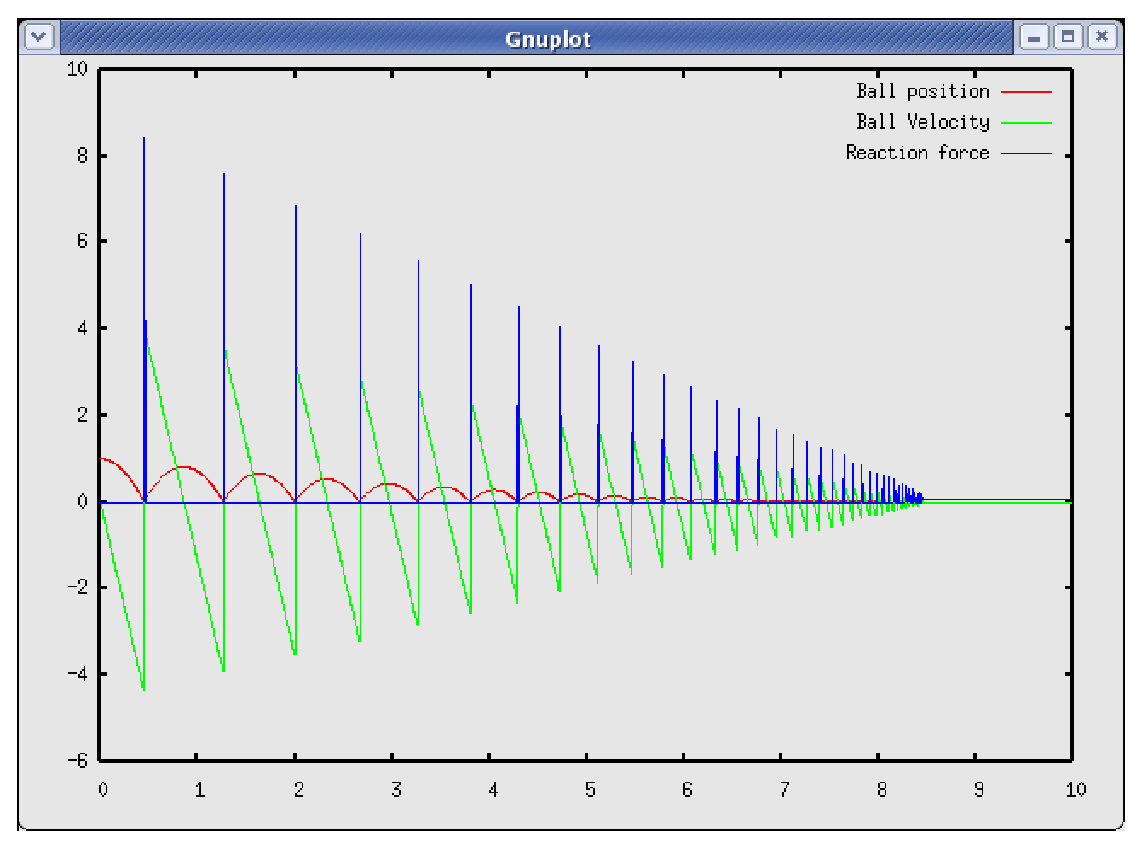
\includegraphics[scale=0.80]{figure/acceptanceTest.ps}
\caption{The bouncing ball}
\label{acceptanceTest}
\end{center}
\end{figure}

\subsubsection{\ac{xml} input file of the bouncing ball test}
\label{BouncingBall_TIDS.xml}
\verbatiminput{BouncingBall_TIDS.xml}


%---------------------------------------------------------------------%
\newpage
\chapter{Quality Assurance Report}
\label{Sec:QR-QAR}

The Quality Assurance Plan is defined in the \ac{paql} document. Corrections and translations of this document will be included in this chapter in the future. 

%---------------------------------------------------------------------%
\newpage
\printglosstex(acr)[p]


%===================================

\listoffigures
\listoftables
\cleardoublepage
%\bibliographystyle{plainnat}
%\bibliography{./Biblio/String,./Biblio/Cp.bib,./Biblio/Optim.bib,./Biblio/Contact.bib,./Biblio/NonSmooth.bib,./Biblio/Leger.bib,./Biblio/Petri.bib}
\cleardoublepage
\end{document}
